\documentclass[11pt,letterpaper]{article}
\usepackage[T1]{fontenc}
\usepackage[utf8]{inputenc}
\usepackage{lmodern}
\usepackage[margin=1in]{geometry}
\usepackage{microtype,amsmath,amssymb,amsthm,mathtools}
\usepackage{graphicx,booktabs,tabularx,array,longtable}
\renewcommand{\tabularxcolumn}[1]{>{\raggedright\arraybackslash}p{#1}}
\usepackage[round,authoryear]{natbib}
\usepackage{xcolor,enumitem,fancyhdr,placeins}
\usepackage[font=small,labelfont=bf]{caption}
\usepackage{url}
\definecolor{navy}{RGB}{23,50,78}
\usepackage[colorlinks=true,linkcolor=navy,citecolor=navy,urlcolor=navy,breaklinks=true]{hyperref}
\hypersetup{pdftitle={The Mathematics of CME},pdfauthor={Miquel Noguer i Alonso},pdfsubject={Futures, implied liquidity, auctions, clearing, margin and delivery}}
\pagestyle{fancy}\fancyhf{}
\fancyhead[L]{\small The Mathematics of CME}
\fancyhead[R]{\small Miquel Noguer i Alonso}
\fancyfoot[C]{\thepage}
\setlength{\headheight}{14pt}
\setlength{\parskip}{3pt}
\setlength{\emergencystretch}{2em}
\renewcommand{\topfraction}{0.9}
\renewcommand{\textfraction}{0.07}
\renewcommand{\floatpagefraction}{0.85}
\setcounter{topnumber}{3}
\setcounter{tocdepth}{1}
\setlist{itemsep=2pt,topsep=4pt}
\numberwithin{equation}{section}
\newtheorem{theorem}{Theorem}[section]
\newtheorem{proposition}[theorem]{Proposition}
\newtheorem{corollary}[theorem]{Corollary}
\newtheorem{lemma}[theorem]{Lemma}
\theoremstyle{definition}
\newtheorem{definition}[theorem]{Definition}
\newtheorem{assumption}[theorem]{Assumption}
\newtheorem{example}[theorem]{Example}
\theoremstyle{remark}
\newtheorem{remark}[theorem]{Remark}
\newcommand{\R}{\mathbb R}
\newcommand{\N}{\mathbb N}
\newcommand{\Z}{\mathbb Z}
\newcommand{\E}{\mathbb E}
\newcommand{\Prob}{\mathbb P}
\newcommand{\ind}{\mathbf 1}
\newcommand{\pos}[1]{\left(#1\right)_+}
\DeclareMathOperator*{\argmax}{arg\,max}
\DeclareMathOperator*{\argmin}{arg\,min}
\DeclareMathOperator{\diag}{diag}
\DeclareMathOperator{\conv}{conv}
\DeclareMathOperator{\VaR}{VaR}
\DeclareMathOperator{\ES}{ES}
\title{\textbf{The Mathematics of CME}\\[5pt]
\large Futures, Implied Liquidity, Auctions, Clearing, and Margin}
\author{Miquel Noguer i Alonso\\[2pt]
 \small Artificial Intelligence Finance Institute (AIFI)}
\date{September 11, 2026\\[4pt]
\small DOI: \href{https://doi.org/10.5281/zenodo.22700054}{10.5281/zenodo.22700054}}
\begin{document}
\maketitle
\begin{abstract}
A futures market allocates contracts, creates linked positions, transfers settlement variation, and constrains those positions through collateral and delivery obligations. This paper develops a mathematical account of these operations in the setting of CME Group's listed derivatives infrastructure. Product-specific matching is represented by integer allocation maps. We establish conservation and rounding bounds for a declared pro-rata stage with FIFO residual allocation, and give an event-fragmentation counterexample. A multiplier-adjusted depth curve measures execution shortfall without treating futures notional as an upfront payment. Implied trading is represented through signed leg vectors and shared resource constraints; a dual certificate explains why individually available implied quantities need not be jointly executable. Observation maps distinguish the exchange state from market-by-order and market-by-price data, while an embedded arrival model links allocation to completion times. Opening price selection, stop election, daily settlement, and final settlement are treated as distinct operations. An exact rounded money-value representation yields a telescoping settlement identity, including changing positions. A separately specified convex scenario-risk model provides margin contours, sensitivity results, and a counterexample to monotonic margin reduction under partial hedge liquidation. Collateral feasibility and minimum funding are characterized by resource and prefix constraints. Options exercise, physical delivery, and a stylized default waterfall complete the lifecycle. Nine reproducible figures and a fully specified numerical ledger connect the results. The contribution is a unified exposition with explicit model boundaries and direct proofs; the illustrative risk functional and allocation routines are not implementations of production SPAN 2 or the complete Globex rule set.
\end{abstract}
\noindent\textbf{Keywords:} futures; CME Globex; pro rata; implied liquidity; auctions; settlement variation; collateral; margin; delivery.
\clearpage
\tableofcontents
\clearpage
\section*{Notation and units}
\addcontentsline{toc}{section}{Notation and units}
\begin{tabularx}{\textwidth}{@{}lX@{}}
\toprule
Symbol & Meaning and units\\
\midrule
$j$, $d$ & Contract index and number of underlying futures contracts.\\
$p_j$, $\tau_j$, $m_j$ & Quote price, permitted price increment, and currency value per price point per contract.\\
$q_i$, $y$, $f_i$ & Resting contracts, aggressor contracts available to a stage, and allocated contracts.\\
$h$, $\rho$ & Integer pro-rata minimum and residual quantity after rounding.\\
$X_n$, $e_n$, $\phi_n$ & Complete modeled state, event, and market phase.\\
$\Pi$, $Y_n$ & Observation map and observed state $\Pi(X_n)$.\\
$a(u)$, $K(Q)$ & Marginal ask price and multiplier-adjusted quote-value integral.\\
$\ell_k$ & Signed underlying-leg vector for one unit of strategy $k$.\\
$A$, $x$, $q$ & Nonnegative recipe-resource matrix, recipe executions, and capacities.\\
$B(p)$, $S(p)$ & Auction-eligible buy and sell quantities at candidate price $p$.\\
$V(p)$, $I(p)$ & Matched volume and signed buy-minus-sell imbalance.\\
$s_t$, $\nu_j(p)$ & Settlement price and rounded money value of one contract.\\
$z_t$, $n_{tk}$ & Signed position after cycle $t$ and signed quantity of trade $k$.\\
$\mathrm{VM}_t$ & Settlement variation for cycle $t$, positive for a receipt.\\
$R(z)$, $M(z)$ & Illustrative scenario risk and total illustrative margin, in currency.\\
$g_s$ & Per-contract loss vector in scenario $s$, in currency.\\
$b_t$, $P_t$ & Free cash and posted cash collateral in the single-currency ledger.\\
$F^*$ & Minimum initial free cash for a specified sequence of cash flows.\\
$c_k$, $a_k$ & Delivery conversion factor and accrued interest in the delivery section.\\
\bottomrule
\end{tabularx}

\medskip
Quantities are integer contracts unless a continuous relaxation is explicitly introduced. Prices may be signed; positivity is not required by the order-book or settlement identities. Monetary examples use U.S. dollars. A quote-value integral is a valuation device, whereas settlement variation is an actual cash flow. The letter $s$ indexes risk scenarios only in the margin section; subscripted $s_t$ denotes a settlement price.

\clearpage
\section{From contract rules to a mathematical state}
\label{sec:foundations}

The natural object of study is the lifecycle of a contract. An order can be admitted yet receive no allocation. A spread can execute while producing several underlying positions. A profitable position can fail a cash deadline. A futures contract can finish trading while leaving a delivery obligation. Each statement concerns a different map, and each map requires a different state.

Throughout this paper, ``CME'' in the title refers to the CME Group listed derivatives setting: Globex trading and the associated clearing infrastructure. CME, CBOT, NYMEX, and COMEX are distinct listing exchanges. The examples identify the relevant exchange rather than treating their contracts as legally interchangeable. Operational anchors are drawn from public specifications and rulebooks consulted on September 11, 2026 (UTC). The principal references are the matching, implied-order, market-data, settlement, risk, and contract sources cited where used.

The mathematical results are elementary or standard consequences of allocation theory, convex analysis, linear programming, and cash-flow accounting. Their purpose is to identify the exact assumptions under which familiar formulas are valid. Convex optimization provides the general background \citep{Boyd2004}; the finite-scenario expected-shortfall representation is attributed separately in Section~\ref{sec:margin}. No empirical estimation, execution advantage, or novelty of those underlying tools is claimed.

\subsection{Contract dimensions}

A contract description contains at least
\begin{equation}
 \kappa_j=(\mathcal P_j,m_j,\text{currency}_j,\text{expiry}_j,
 \text{settlement}_j,\text{delivery}_j,\text{algorithm}_j),
\end{equation}
where $\mathcal P_j$ is the applicable price grid. The grid may depend on order form or price range. It is not always correct to infer the tick of a spread or option from the tick of its underlying outright.

\begin{table}[htbp]
\centering\small
\begin{tabularx}{\textwidth}{@{}lXXX@{}}
\toprule
Contract & Listing exchange & Value factor and outright tick & End obligation\\
\midrule
E-mini S\&P 500 (ES) & CME & \$50/point; 0.25 point, or \$12.50 & Cash settlement\\
Light Sweet Crude Oil (CL) & NYMEX & 1,000 barrels; \$0.01/barrel, or \$10 & Physical delivery\\
Treasury note (Chapter 19) & CBOT & \$1,000/point; $1/64$ point, or \$15.625 before currency rounding & Deliverable Treasury notes\\
\bottomrule
\end{tabularx}
\caption{Selected dimensions, not a universal product template. Sources: \citet{CME358,NYMEX200,CBOT19}. The Treasury amount illustrates why quote increments and banked currency amounts must be distinguished.}
\label{tab:contracts}
\end{table}

For example, one ES contract at 6,000 points has a reference notional of \$300,000. A one-point change generates \$50 of linear mark-to-market exposure per contract. The trade does not require a \$300,000 purchase payment. Performance-bond transfers, variation, fees, and possible final obligations belong in a separate cash ledger. This distinction will prevent a false execution-cost interpretation in Section~\ref{sec:depth}.

\subsection{The state and its transitions}

Let event time be $n=0,1,\ldots$. A sufficiently detailed modeled state is
\begin{equation}
 X_n=(\mathcal O_n,\mathcal H_n,\mathcal G_n,\phi_n,
       \kappa_n,z_n,b_n,P_n,\theta_n).
\label{eq:state}
\end{equation}
Here $\mathcal O$ contains working orders and priority, $\mathcal H$ contains hidden or contingent interest, $\mathcal G$ records enabled implication recipes and their inputs, and $\phi$ is market phase. Positions $z$, cash $b$, and collateral $P$ are indexed by account when necessary. The parameter state $\theta$ contains quantities such as risk parameters, admissibility restrictions, settlement references, and outstanding deadlines. This is a modeling construction, not a description of CME's internal database.

An accepted event acts through
\begin{equation}
 X_{n+1}=T_{e_n}(X_n),\qquad
 \mathcal L_{n+1}=\mathcal L_n\mathbin{\|}\Delta\mathcal L(e_n,X_n),
\end{equation}
where $\mathcal L$ is the ledger and $\|$ appends the new records. A useful ledger preserves the distinction between an order acknowledgment, an execution, an underlying-leg position change, a valuation, and a cash transfer. For example, computing a settlement price changes the valuation reference; the associated banked variation is a separate accounting operation.

\begin{assumption}[Declared numerical scope]\label{ass:scope}
Unless stated otherwise, examples use ordinary displayed limit orders, exact integer quantities, no self-match restrictions, no cancellations during a match, no hidden replenishment, and no special priority entitlement. Products, recipe sets, and market phases are held fixed during each calculation. Fees and interest are zero in the numerical ledger. These are assumptions of the examples, not claims about all trading on Globex.
\end{assumption}

The scope matters. A proof for a price-time queue does not establish a result for a TOP stage or an LMM stage. A constraint on final cash does not establish that intermediate calls can be met. A net position across several accounts does not establish that the accounts may share collateral.

\subsection{Conservation at three levels}

For a trade in a single future, signed position changes sum to zero across counterparties. For a strategy, this holds separately for every underlying leg. If all accounts use the same settlement-value map, variation also sums to zero before fees and other external flows. Collateral movements preserve an individual account's total assets only when both the free and posted sides are included. These are different conservation statements; none implies that every participant has sufficient liquid cash at every deadline.

The rest of the paper develops these maps in lifecycle order. Matching and depth determine executions. Implication links books. Observation limits inference. Opening changes the matching phase. Settlement changes cash. Risk and collateral constrain continuation. Delivery and exercise determine the remaining obligations.
\FloatBarrier

\section{Integer matching and allocation}
\label{sec:allocation}

Globex supports several matching families. FIFO, pro rata, TOP, LMM, and configurable combinations have different roles; the assigned product configuration determines which stages apply. A generic ``CME pro-rata formula'' is therefore insufficient. The public algorithm matrix supplies the order of stages, while the step documentation specifies their local behavior \citep{CMEMatching,CMESteps}.

\subsection{Price selection and allocation are different maps}

Let a buy aggressor have remaining size $Q$ and limit $L$. First identify the best eligible opposite price, including eligible implication. At a selected price, let $q=(q_1,\ldots,q_n)$ be the quantities available to the relevant allocation stage. The stage produces
\begin{equation}
 f=\mathcal A(q,y;\vartheta),\qquad
 0\le f_i\le q_i,\quad \sum_i f_i\le y,
\end{equation}
where $\vartheta$ contains that stage's configuration and $y$ is its available aggressor quantity. A later stage operates on updated remaining quantities. The proportions in a later pro-rata step must therefore use its own input state, rather than the original book automatically.

For a declared stage with sufficient compatible resting quantity, complete allocation requires $\sum_i f_i=y$. The public step description also identifies a FIFO exception when aggressing quantity exceeds available resting quantity. In the ordinary displayed examples here, that exception exhausts the available orders. We do not model the ordering of individual execution reports in that branch.

\subsection{FIFO as a prefix operator}

Order the eligible ordinary orders first by best price and then by applicable time priority. Define $H_i=\sum_{j\le i}q_j$, with $H_0=0$. The FIFO fill is
\begin{equation}
 f_i(Q)=\min\{q_i,(Q-H_{i-1})_+\}.
\label{eq:fifo}
\end{equation}

\begin{proposition}[FIFO conservation and composition]\label{prop:fifo}
Under Assumption~\ref{ass:scope}, FIFO fills $\min(Q,H_n)$ contracts and never fills a later order while leaving available quantity ahead of it. Two consecutive aggressors with the same side and limit, sizes $Q_1,Q_2$, and no intervening state change have the same total order-level fills as one aggressor of size $Q_1+Q_2$.
\end{proposition}
\begin{proof}
Represent order $i$ by the interval $(H_{i-1},H_i]$ on a quantity axis. Its fill is the length of its intersection with $(0,Q]$. The intersections partition $(0,\min(Q,H_n)]$, establishing conservation and priority. The first aggressor removes a prefix. The second removes the next prefix of the residual list. Their union is the prefix of length $\min(Q_1+Q_2,H_n)$.
\end{proof}

The interval argument fails if a new event refreshes hidden display, changes priority, or elects additional interest. CME's FIFO modification documentation identifies working-size increases, price changes, and account-number changes as priority-losing amendments \citep{CMESteps}. The composition statement deliberately excludes amendments and replenishment.

\subsection{A pro-rata stage with an integer minimum}

We now specify one complete model: a pro-rata step with integer minimum $h\ge1$, followed by ordinary FIFO residual allocation, with no TOP, LMM, split, or leveling step. Working quantities mean eligible displayed quantities in this model. Let
\begin{equation}
 Q_0=\sum_iq_i>0,\qquad 0\le y\le Q_0,\qquad
 w_i=\frac{yq_i}{Q_0}.
\end{equation}
The first-pass allocation and residual are
\begin{equation}
 b_i=\begin{cases}\lfloor w_i\rfloor,&\lfloor w_i\rfloor\ge h,\\
 0,&\lfloor w_i\rfloor<h,
 \end{cases}
 \qquad \rho=y-\sum_i b_i.
\label{eq:prbase}
\end{equation}
Apply FIFO to residual capacities $q_i-b_i$ with size $\rho$ to obtain $r_i$; finally $f_i=b_i+r_i$. Thresholding the integer part is equivalent to testing $w_i\ge h$ because $h$ is an integer. This model follows the documented minimum-and-rounding structure \citep{CMESteps}, but is not an implementation of every supported algorithm.

\begin{proposition}[Conservation and discrepancy]\label{prop:rounding}
The above allocation is well defined and satisfies
\begin{equation}
 \sum_i f_i=y,\quad 0\le f_i\le q_i,\quad
 0\le\rho<nh,\quad
 \sum_i|f_i-w_i|\le2\rho<2nh.
\end{equation}
\end{proposition}
\begin{proof}
Since $y\le Q_0$, $b_i\le w_i\le q_i$. If $b_i=0$, then $0\le w_i<h$. Otherwise $0\le w_i-b_i<1\le h$. Summing gives $\rho=\sum_i(w_i-b_i)\in[0,nh)$. Residual capacity is $Q_0-\sum_i b_i\ge\rho$, so FIFO allocates the entire residual without exceeding capacity. Write $d_i=w_i-b_i\ge0$. Then $f_i-w_i=r_i-d_i$, with $\sum_i r_i=\sum_i d_i=\rho$. The triangle inequality gives the claimed bound.
\end{proof}

This is a bound on departure from the fractional allocation of a \emph{single stage}. It is not a guarantee that final allocations of a multi-stage algorithm are approximately proportional. A priority stage may intentionally allocate a large fraction to one order. When $y=Q_0$, the final vector is $q$ regardless of how the intermediate rounding is organized.

\begin{table}[htbp]
\centering
\begin{tabular}{@{}lrrrrr@{}}
\toprule
Order & Resting size & Fractional $w_i$ & PR base & PR + FIFO & FIFO\\
\midrule
1 & 12 & 4.44 & 4 & 5 & 12\\
2 & 28 & 10.36 & 10 & 10 & 25\\
3 & 60 & 22.20 & 22 & 22 & 0\\
\midrule
Total & 100 & 37.00 & 36 & 37 & 37\\
\bottomrule
\end{tabular}
\caption{A 37-contract aggressor at one price, $h=2$, and orders listed in FIFO order. All prices are identical, so allocation changes who fills without changing this aggressor's execution price.}
\label{tab:allocation}
\end{table}

\subsection{Fragmentation changes the mechanism's input}

\begin{example}[No general event-composition law]\label{ex:fragment}
Take $q=(2,3,5)$ and $h=2$. For a single aggressor of size four, $w=(0.8,1.2,2)$, the PR base is $(0,0,2)$, and the two residual contracts go to the first order. Thus $f=(2,0,2)$.

Instead submit two consecutive aggressors of size two. On the first, no fractional entitlement reaches two, so FIFO allocates $(2,0,0)$. Remaining sizes are $(0,3,5)$. On the second, entitlements are $(0,0.75,1.25)$, again all below two. FIFO gives $(0,2,0)$. Total fills are $(2,2,0)$.
\end{example}

The difference is caused by the reset of the proportional calculation at the next event. A simulator that merges the two aggressors changes the result even though total quantity, side, and price are unchanged. Similarly, replacing the $h=2$ minimum by $h=1$ in the single-event example gives $(1,1,2)$ rather than $(2,0,2)$.

\begin{figure}[htbp]
\centering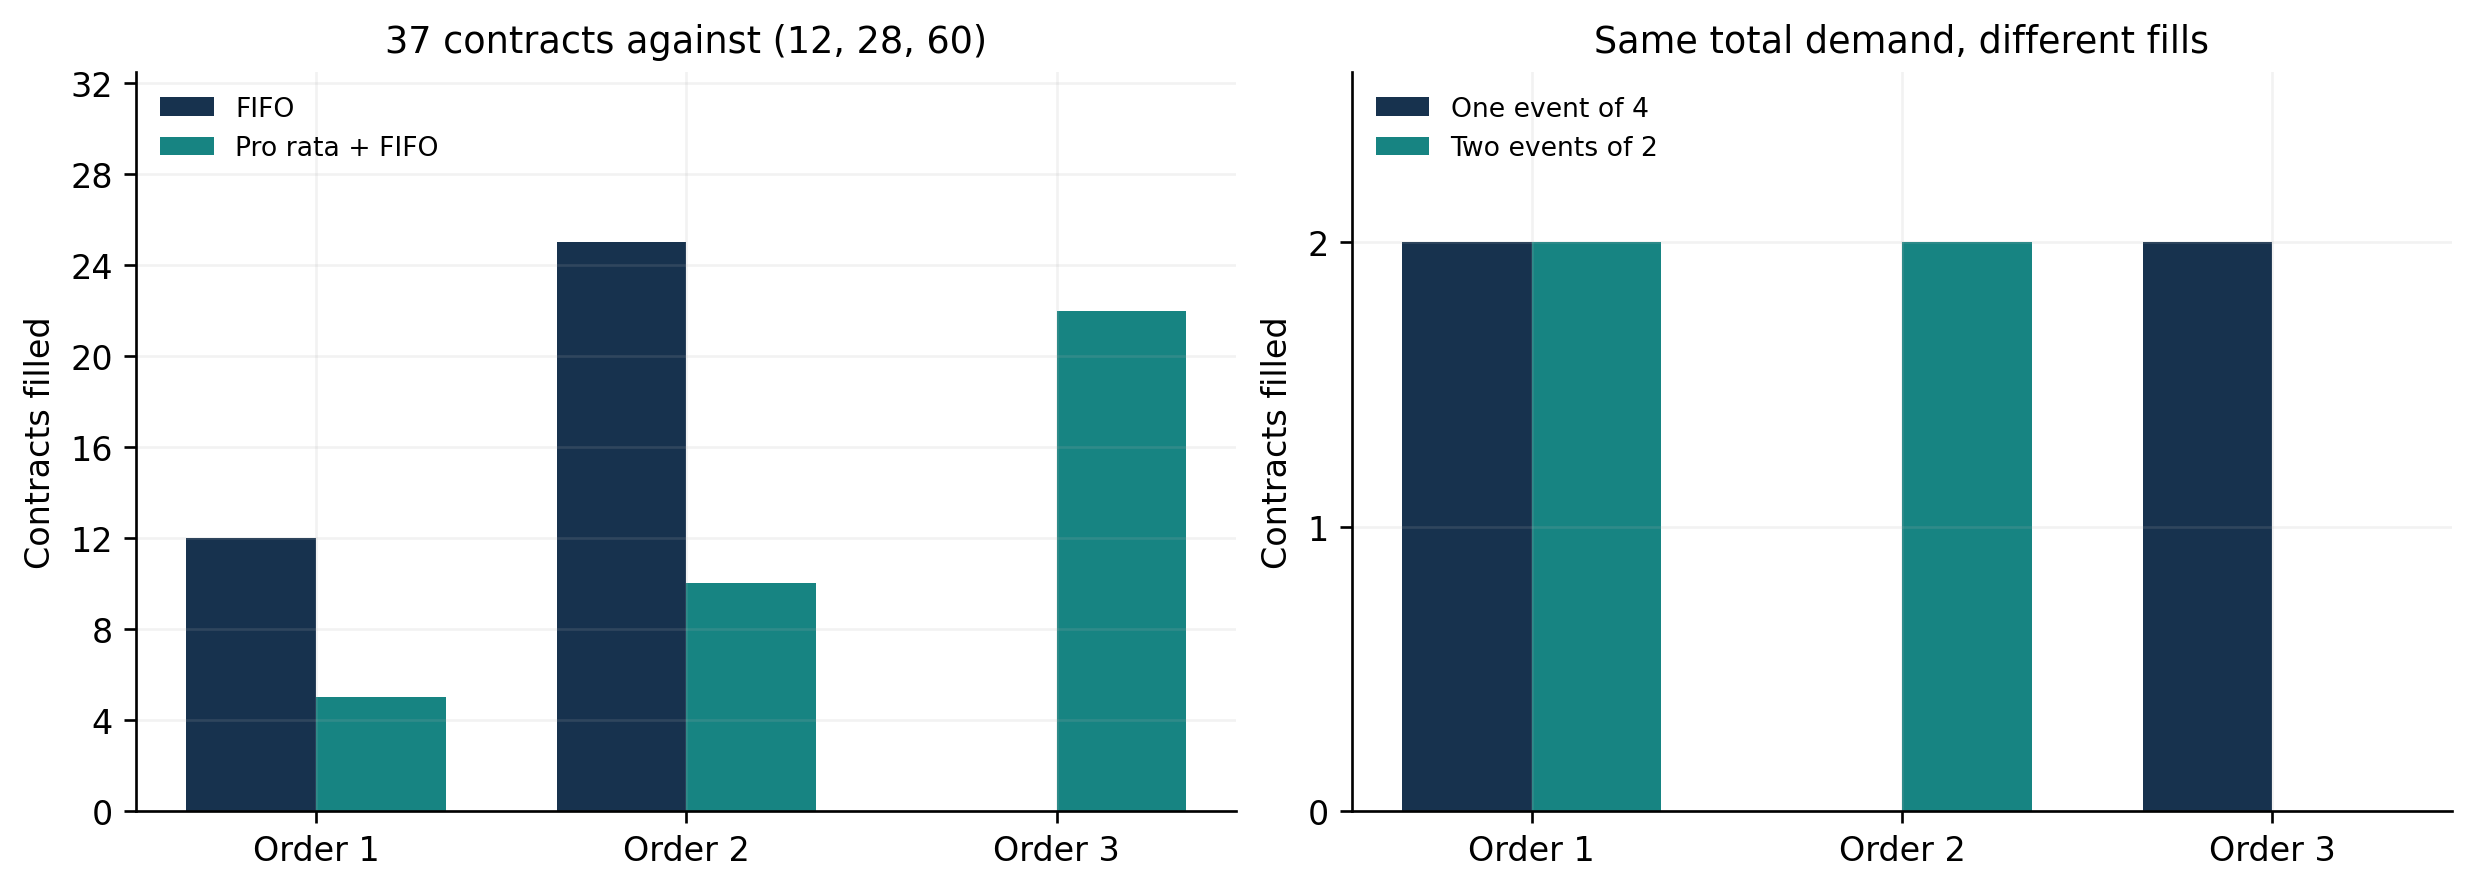
\includegraphics[width=\textwidth]{figures/01_allocation.png}
\caption{Allocation effects isolated from price effects. Left: Table~\ref{tab:allocation}. Right: Example~\ref{ex:fragment}. Contract conservation holds in every bar group; participant outcomes differ.}
\label{fig:allocation}
\end{figure}

\subsection{What a configurable model must preserve}

It is useful to write a configured allocator as a composition of stages, but the composition operates on both remaining demand and remaining book state:
\begin{equation}
 (q^{k+1},y^{k+1},\eta^{k+1})
 =T_k(q^k,y^k,\eta^k),
\end{equation}
where $\eta$ contains entitlement and priority information. Stage order, eligibility, integer rounding, and residual handling are all part of $T_k$. The configurable family includes optional leveling after proportional allocation; it must not be silently replaced by the FIFO residual model above \citep{CMEMatching}. We do not assign undocumented entitlement percentages to a named product.

The right abstraction is therefore a family of allocation maps indexed by configuration and market phase. Contract conservation survives across the family when each stage is conservative. FIFO composition and proportional discrepancy bounds require their additional assumptions.
\FloatBarrier

\section{The geometry of depth in contract units}
\label{sec:depth}

\subsection{A marginal execution-price curve}

Fix a contract and a frozen list of eligible ordinary asks. At distinct prices $p_1<\cdots<p_k$, let available quantities be $q_1,\ldots,q_k$. Set $H_i=\sum_{j\le i}q_j$ and $H_0=0$. On the quantity interval $(0,H_k]$, define
\begin{equation}
 a(u)=p_i\quad\text{for }H_{i-1}<u\le H_i,
 \qquad K(Q)=m\int_0^Q a(u)\,du.
\label{eq:depth}
\end{equation}
For integer $Q$, this is the multiplier times the sum of the executed quote prices. Interpolation to real $Q$ is a mathematical device. It neither creates fractional contracts nor relaxes exchange lot constraints.

\begin{proposition}[Convex quote-value geometry]\label{prop:depth}
For $0\le Q\le H_k$, $K$ is continuous, piecewise linear, and convex. At an interior depth boundary $H_i$,
\begin{equation}
 \partial K(H_i)=[mp_i,mp_{i+1}],
 \qquad K''=m\sum_{i=1}^{k-1}(p_{i+1}-p_i)\delta_{H_i}
\end{equation}
in the distributional sense. The average execution price $K(Q)/(mQ)$ is nondecreasing for $Q>0$.
\end{proposition}
\begin{proof}
The derivative away from depth boundaries is $ma(Q)$, a nondecreasing step function. Its jumps are exactly $m(p_{i+1}-p_i)$, which establishes convexity, the subdifferential, and the distributional formula. Increasing $Q$ appends contracts whose prices are at least the average of the existing prefix. The average therefore cannot fall.
\end{proof}

No assumption that futures prices are positive is needed. If prices are negative, $K$ can decrease while remaining convex. What is increasing is the marginal price, not necessarily the level of the quote-value integral.

\subsection{Shortfall is a relative valuation}

Against benchmark price $p_0$, define buy execution shortfall
\begin{equation}
 \mathrm{IS}(Q;p_0)=K(Q)-mQp_0.
\label{eq:is}
\end{equation}
If all $Q$ purchased contracts remain open to a settlement $s$, their linear variation is
\begin{equation}
 \mathrm{VM}=mQs-K(Q)
 =mQ(s-p_0)-\mathrm{IS}(Q;p_0).
\label{eq:shortfallvm}
\end{equation}
Thus shortfall reduces the eventual marked gain by an exact dollar amount. It is not the initial margin deposit, and $K(Q)$ is not a bank debit at trade entry. Section~\ref{sec:settlement} gives the currency-rounded version and permits subsequent trades.

\begin{example}[An ES depth walk]\label{ex:depth}
Use ES asks of three contracts at 6,000.00, five at 6,000.25, and four at 6,000.50. A ten-contract buy fills $(3,5,2)$. With $m=50$,
\begin{align}
 K(10)&=50(3\cdot6000+5\cdot6000.25+2\cdot6000.50)\notag\\
      &=\$3{,}000{,}112.50,\\
 \bar p&=6000.225,\qquad
 \mathrm{IS}(10;6000)=\$112.50.
\end{align}
An average fill price need not itself lie on the order-entry grid. If the settlement is 6,001.00, the position receives \$387.50 in variation before fees: a \$500 benchmark gain less \$112.50 of execution shortfall.
\end{example}

\begin{figure}[htbp]
\centering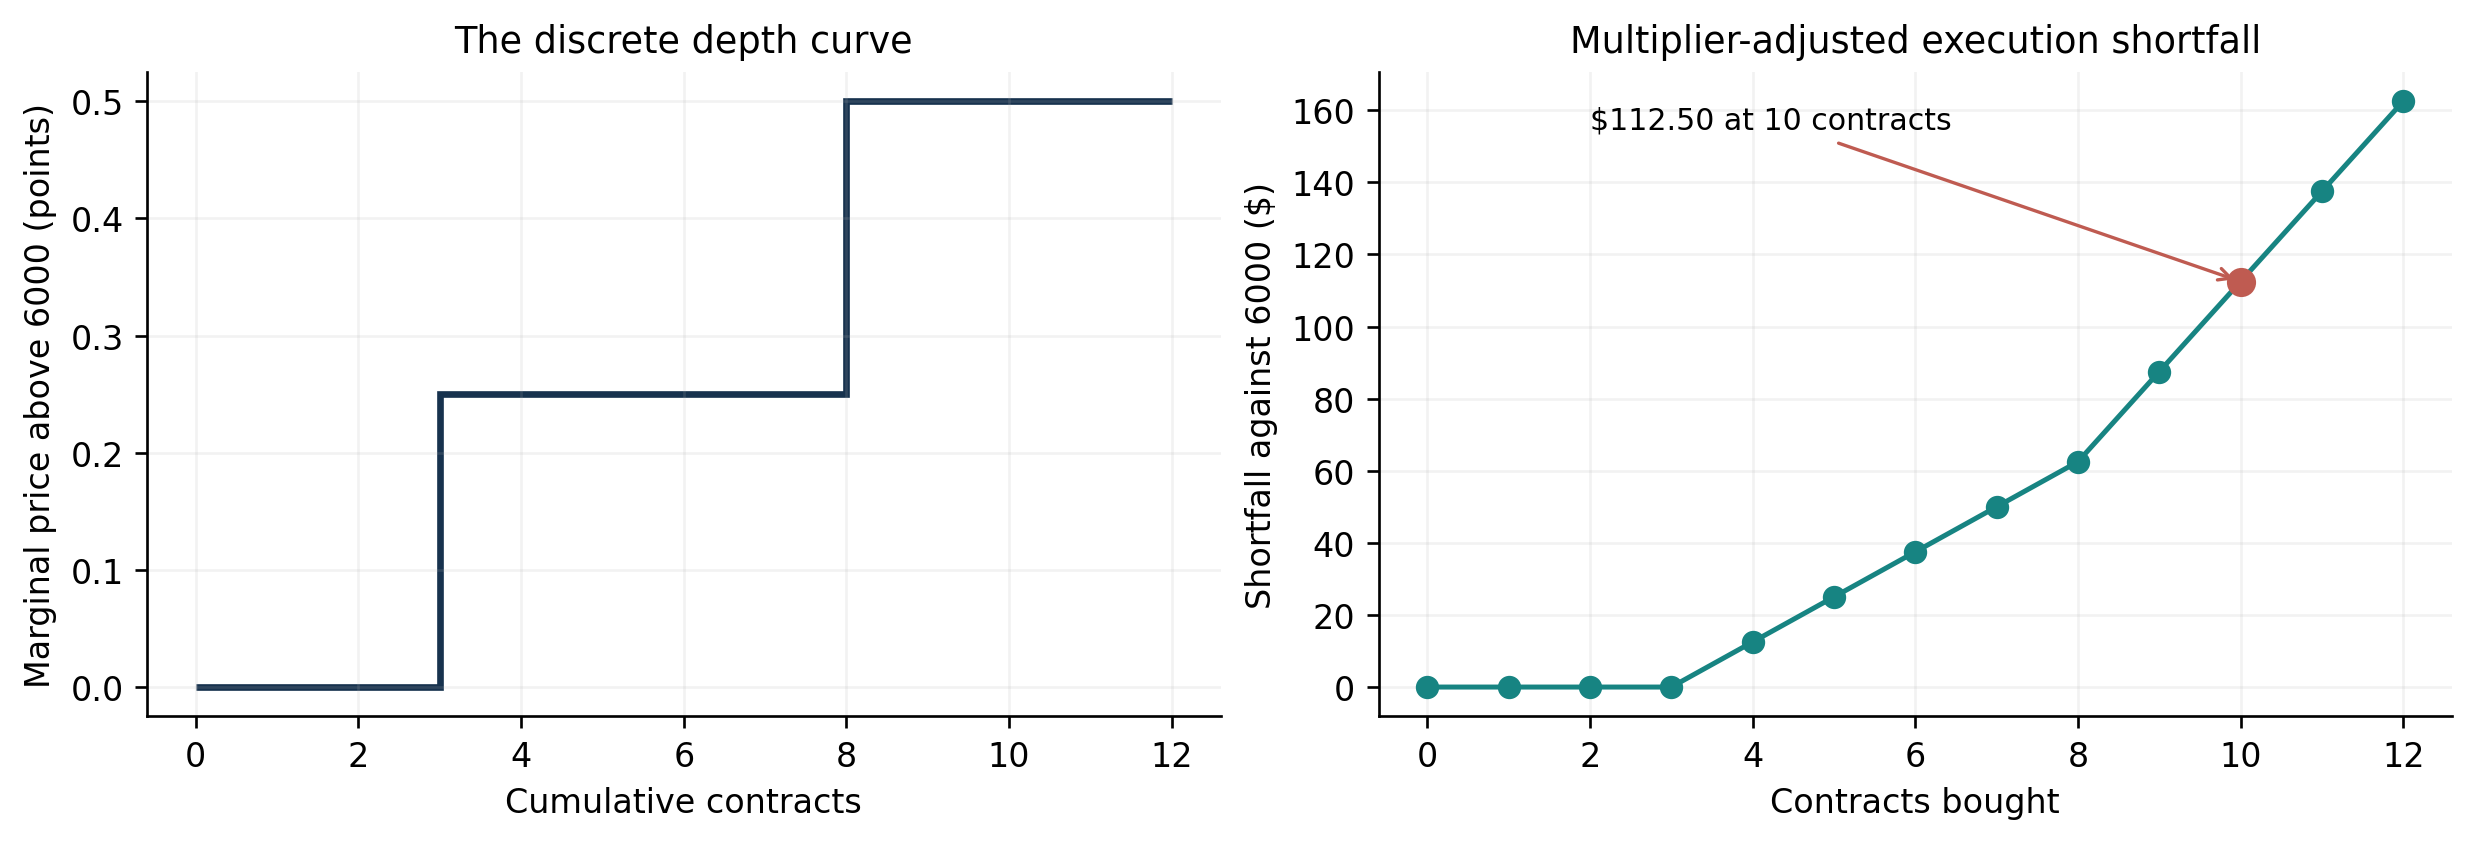
\includegraphics[width=\textwidth]{figures/02_depth.png}
\caption{The depth curve and execution shortfall in Example~\ref{ex:depth}. The slopes of the shortfall curve are the marginal price differences multiplied by \$50 per point.}
\label{fig:depth}
\end{figure}

\subsection{Price limits and perturbations}

\begin{corollary}[Buy-limit monotonicity]\label{cor:limit}
For a fixed quantity and a frozen ordinary book ranked first by price, increasing a buy limit cannot decrease the fill. If the original fill is positive, its average execution price weakly increases.
\end{corollary}
\begin{proof}
Newly eligible asks are appended after the original eligible list. Original fills are unchanged, and any additional contracts have prices at least as high as every originally eligible price. If no additional contracts fill, the average is unchanged; otherwise it is a weighted average of the original average and a weakly higher average.
\end{proof}

The assumptions exclude changes to implication, compatibility, and price controls during the match. With such changes, the eligible list itself must first be recomputed.

For two marginal curves $a,\widehat a$ on a common quantity interval,
\begin{equation}
 |K(Q)-\widehat K(Q)|
 \le m\int_0^Q|a(u)-\widehat a(u)|\,du.
\label{eq:depthbound}
\end{equation}
In particular a uniform price error $\delta$ yields a dollar error at most $mQ\delta$. This estimate exposes the importance of units: the same quote error has different financial consequences for contracts with different value factors. It also says nothing about queue priority, fill probability, or whether several implied quotes can be consumed simultaneously. Those are different parts of the state.
\FloatBarrier

\section{Implied liquidity as a constrained network}
\label{sec:implied}

An implied-IN opportunity combines outright orders to offer a spread; an implied-OUT opportunity combines a spread with other legs to offer an outright. CME documents both constructions. It also specifies that implied bids do not trade directly against implied offers, that implication is unavailable in nonmatching phases, and that some executable implied quantities are not disseminated \citep{CMEImplied}. Consequently, neither an unrestricted network optimizer nor a sum of displayed quantities is a faithful description of the mechanism.

\subsection{Signed legs and quote conventions}

Let $e_j$ be the unit vector for underlying future $j$. A strategy is described by an integer leg vector $\ell\in\Z^d$. Buying a one-for-one calendar $A-B$ creates
\begin{equation}
 \ell_{AB}=e_A-e_B.
\end{equation}
With common multiplier $m$, its difference quote is $p_A-p_B$ and its signed underlying quote value is $m(p_A-p_B)$. With unequal multipliers, currencies, or ratio conventions, the conversion must instead be performed leg by leg. A raw subtraction of two displayed numbers need not be financially meaningful.

For strategy executions $x_k\in\N$,
\begin{equation}
 \Delta z=\sum_kx_k\ell_k=Lx,
 \qquad L=[\ell_1\ \cdots\ \ell_K].
\label{eq:legs}
\end{equation}
The matrix $L$ records signed positions. It is distinct from the nonnegative matrix that records consumption of available orders.

\subsection{Recipes consume shared inputs}

Enumerate a \emph{declared} set of feasible matching recipes $k=1,\ldots,K$. A recipe includes its aggressor form, required resting orders, prices, leg ratios, and phase eligibility. Let $A_{ik}$ be the number of contracts consumed from resting order $i$ per unit of recipe $k$. With available capacities $q_i$, any execution vector must satisfy
\begin{equation}
 x\in\Z_+^K,\qquad Ax\le q.
\label{eq:resources}
\end{equation}
This is a necessary resource condition. It is sufficient only for the explicitly declared simultaneous-allocation model with no further compatibility or sequencing restrictions. The exchange chooses according to its priority rules; it is not asserted to solve a global maximum-volume integer program.

\begin{example}[Eleven indicated contracts, eight jointly feasible]\label{ex:shared}
Consider three CL maturities and ordinary resting orders: an $A$ ask for eight contracts at 75.01, a $B$ bid for five at 74.81, and a $C$ bid for six at 74.51. All prices are dollars per barrel. There is an implied ask for five $A-B$ spreads at 0.20 and an implied ask for six $A-C$ spreads at 0.50. In the restricted recipe model,
\begin{equation}
 A=\begin{pmatrix}1&1\\1&0\\0&1\end{pmatrix},\quad
 q=\begin{pmatrix}8\\5\\6\end{pmatrix},\quad
 x_1\le5,\quad x_2\le6,\quad x_1+x_2\le8.
\end{equation}
Five plus six is eleven, but both constructions use the same $A$ ask. At most eight spread contracts can execute jointly. The allocation $(x_1,x_2)=(5,3)$ consumes $(8,5,3)$ underlying contracts and creates aggressor positions $(8,-5,-3)$.
\end{example}

The signed entry quote value for that allocation is
\begin{equation}
 1000[8(75.01)-5(74.81)-3(74.51)]
 =1000[5(0.20)+3(0.50)]=\$2{,}500.
\end{equation}
This is a difference valuation for the leg ledger, not an upfront premium. Its subsequent variation depends on the settlement changes of all three maturities.

An implied-OUT calculation in a separate matching opportunity is equally direct: an $A-B$ ask at 0.20 for four contracts and a $B$ ask at 74.82 for seven imply an $A$ ask at 75.02 for at most four. The signs are essential: buying the spread gives $+A-B$, and buying $B$ cancels the $-B$ leg. Two sell orders in unrelated maturities would not produce this exposure.

\begin{figure}[htbp]
\centering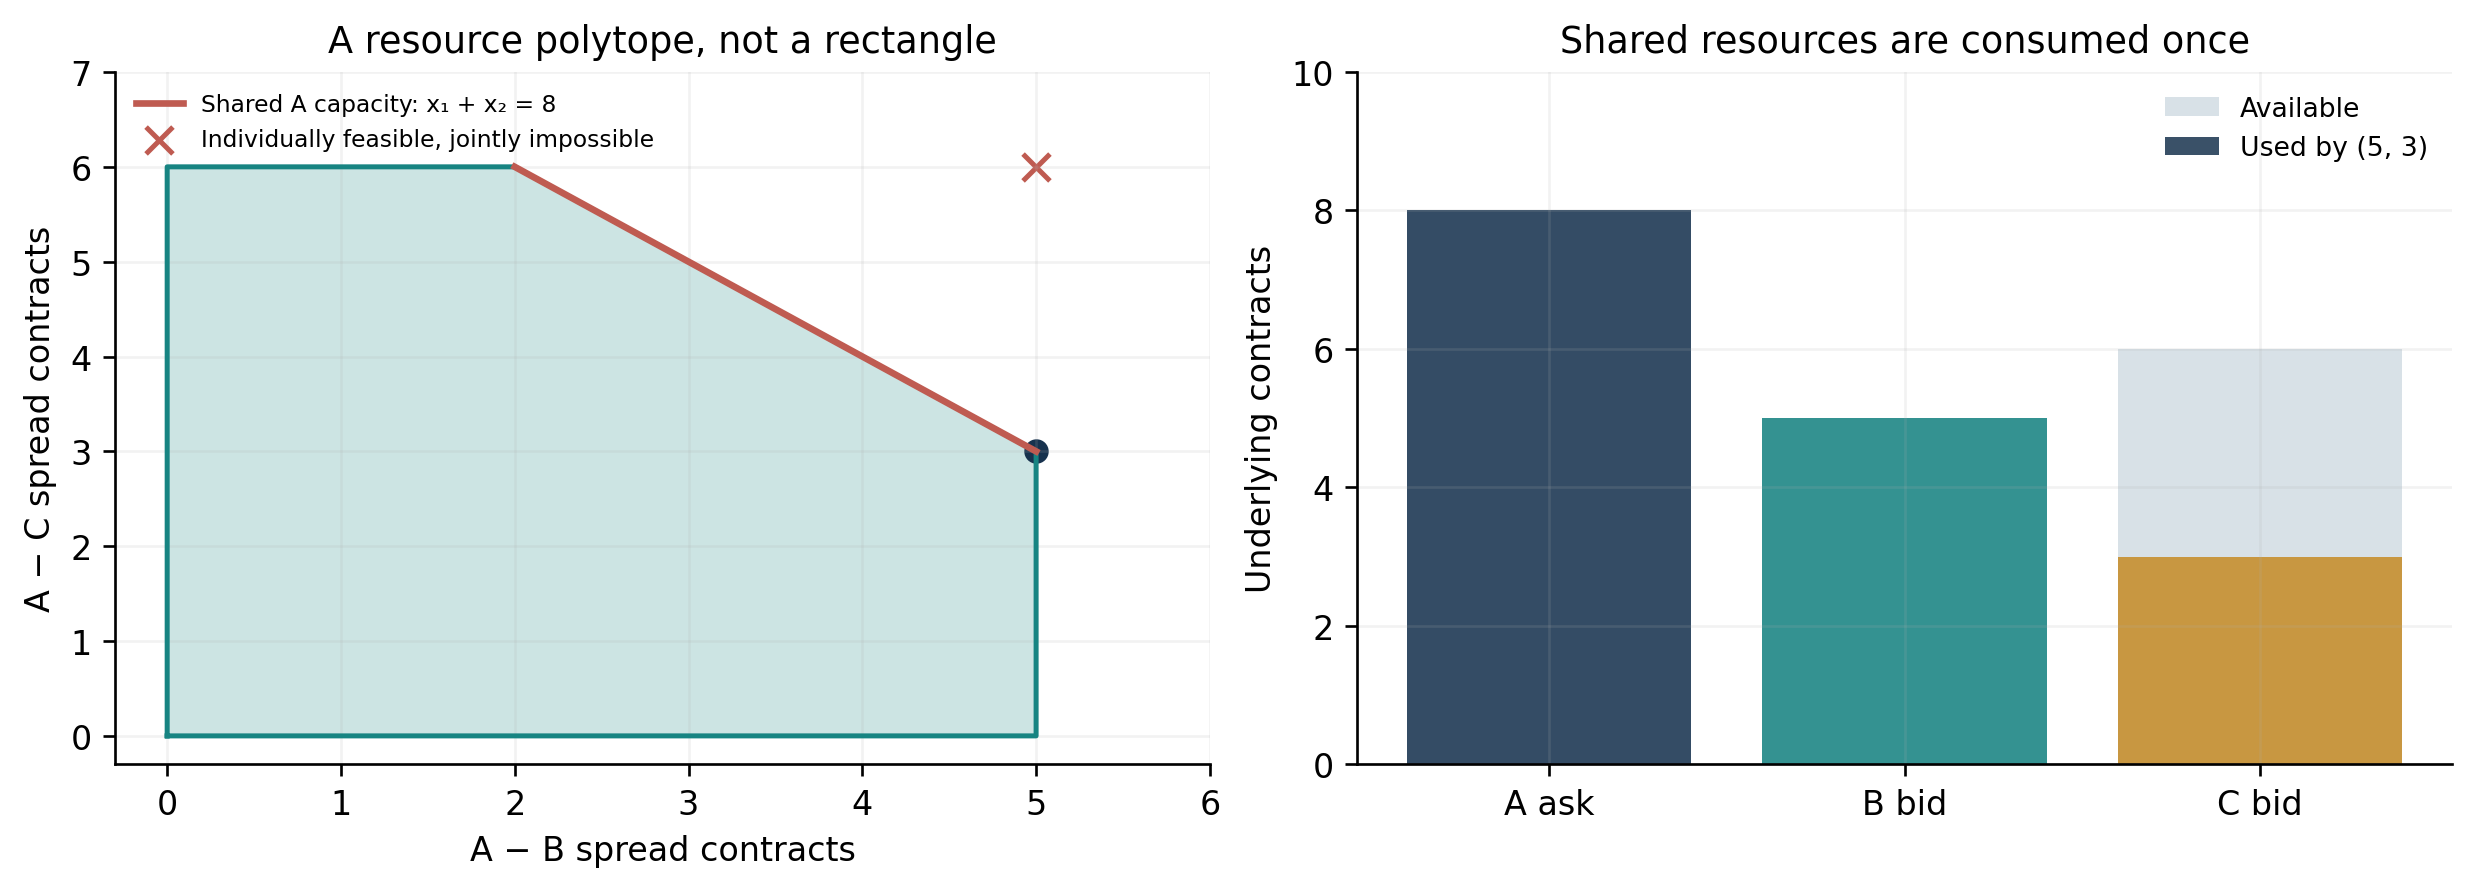
\includegraphics[width=\textwidth]{figures/03_implied.png}
\caption{Shared-resource geometry in Example~\ref{ex:shared}. The feasible polygon removes the upper-right corner of the rectangle suggested by individual implied quantities. The point $(5,6)$ is infeasible; $(5,3)$ uses the common $A$ capacity exactly.}
\label{fig:implied}
\end{figure}

\subsection{A dual certificate for available liquidity}

For nonnegative recipe weights $w_k$, consider the continuous relaxation
\begin{equation}
 \max\{w^\top x:Ax\le q,\ x\ge0\}.
\label{eq:primal}
\end{equation}
Weights may measure spread lots in a common unit or another declared objective. Counting unrelated multi-leg strategies as if one unit meant the same exposure is not generally useful.

\begin{proposition}[Resource-price certificate]\label{prop:dual}
For any $\lambda\ge0$ satisfying $A^\top\lambda\ge w$, every feasible integer or real allocation satisfies
\begin{equation}
 w^\top x\le\lambda^\top q.
\end{equation}
If a feasible $x^*$ and such a $\lambda^*$ attain equality, both certify the optimum of the relaxation, and $x^*$ is also integer-optimal if integer valued.
\end{proposition}
\begin{proof}
Nonnegativity gives $w^\top x\le\lambda^\top Ax\le\lambda^\top q$. Equality at a feasible pair leaves no room for improvement.
\end{proof}

In Example~\ref{ex:shared}, $w=(1,1)$ and $\lambda=(1,0,0)$ give the upper bound eight. The feasible integer point $(5,3)$ attains it. The entire bottleneck is certified by the shared $A$ order. In more general ratio systems, the relaxation need not be integral; its value remains an upper bound and must not be reported as an executable contract count without an integer solution.

\subsection{Price potentials and cycles}

For maturities with a common price convention, assign a scalar potential $p_j$ to each vertex and difference quote $c_{ij}=p_i-p_j$ to a calendar edge. For any closed cycle,
\begin{equation}
 c_{12}+c_{23}+\cdots+c_{k1}=0.
\label{eq:cycle}
\end{equation}
Conversely, on a connected graph, antisymmetric edge values with zero sum around every cycle admit vertex potentials, unique up to an additive constant. To construct them, fix one vertex value and sum edge differences along a path; zero cycle sums make the result path independent.

This identity describes consistent difference valuations. For actual bid and ask executions, the corresponding no-arbitrage statement requires a \emph{jointly feasible} zero-net-leg trade cycle, correct multipliers, fees, and settlement conventions. If its signed entry value is negative and its net position is zero, the settlement identity in Section~\ref{sec:settlement} converts the negative entry value into a positive gain before costs. A displayed cycle with insufficient shared capacity or disallowed implied-to-implied matching provides no such executable transaction.

The topology therefore has two layers: signed exposure describes what a strategy creates, and nonnegative capacity describes which strategies can coexist. A useful model preserves both.
\FloatBarrier

\section{Observation, event time, and completion}
\label{sec:observation}

\subsection{A feed is a projection}

CME's futures and options market-data documentation distinguishes market-by-price, market-by-order full-depth, and implied-book information \citep{CMEMDP}. A public view is written
\begin{equation}
 Y_n=\Pi(X_n).
\end{equation}
The map $\Pi$ can discard reserve size, unelected stops, account information, recipe inputs, or other attributes. An order identifier is not a participant identity. A full-depth order view does not imply full knowledge of the state in \eqref{eq:state}.

For the documented MBO view, ordering first uses instrument, side, and price, and then the order-priority value within the same price and side. Lower priority numbers rank ahead locally. The priority field is supplied regardless of the product's matching algorithm, and implied-book information is not transmitted in MBO format \citep{CMEMBO}. It follows that sorting an MBO book gives an observed order sequence; it does not convert every product into a FIFO allocation market.

\begin{proposition}[When an observed transition exists]\label{prop:projection}
Fix a deterministic event map $T_e$. There exists a map $\widetilde T_e$ on observed states with
\begin{equation}
 \Pi T_e=\widetilde T_e\Pi
\end{equation}
if and only if $\Pi T_e(x)=\Pi T_e(x')$ whenever $\Pi(x)=\Pi(x')$.
\end{proposition}
\begin{proof}
If $\widetilde T_e$ exists, equal observations have the same image under it. Conversely, define $\widetilde T_e(y)=\Pi T_e(x)$ for any $x$ with $\Pi(x)=y$. The stated condition makes this definition independent of the representative $x$.
\end{proof}

For a concrete failure, two books have the same price-level total ten and two orders. In one, order A has size two and order B size eight; in the other, A and B each have size five. Cancel A. Remaining price-level depth is eight in the first book and five in the second. Aggregated depth alone cannot determine the update even though the cancellation is unambiguous at order level.

A related failure occurs with hidden interest: two books may expose the same displayed order while carrying different reserves. Their observations can agree until a depletion event refreshes one of them. This does not contradict reconstruction of the displayed book; it limits what that reconstruction identifies.

\subsection{Complete events, not arbitrary message prefixes}

The CME event documentation groups messages generated by order actions and state changes, and provides the MatchEventIndicator to identify the event boundary. An event can include trades, book changes, and implied-quote changes; some events, such as entry of an unelected stop, need not produce public market data \citep{CMEEvents}.

Suppose a single matching event consumes an order that supports two implied quotes. An observer may receive a trade update, a direct-book update, and an implied update at different moments. A partial message prefix can temporarily combine a depleted direct order with its old implied quantities. Treating that prefix as a simultaneous executable state creates fictitious liquidity. Complete-event processing resolves this particular inconsistency, although it does not recover hidden state or eliminate network latency.

Let $\mathcal F_t^{\rm obs}$ be the information available after valid event completion and applicable recovery. A model should distinguish the last valid observation from an interval with an unresolved gap. Filling a sequence gap with a zero-change assumption creates data that were never observed. The numerical code accompanying this paper begins from synthetic complete states; it does not claim to decode MDP packets or implement recovery.

\subsection{The allocation map changes completion time}

To isolate allocation from order-arrival uncertainty, consider a static book repeatedly hit by same-price aggressors of fixed batch size $b$. Let the arrival count $N_t$ be a Poisson process with rate $\lambda>0$. At each arrival apply one declared allocation map, update remaining quantities, and continue. There are no competing orders or cancellations.

\begin{proposition}[An embedded-event completion law]\label{prop:erlang}
If order $i$ completes at deterministic arrival index $k_i$, then its completion time $T_i$ satisfies
\begin{equation}
 \Prob(T_i\le t)=\Prob(N_t\ge k_i)
 =1-e^{-\lambda t}\sum_{j=0}^{k_i-1}\frac{(\lambda t)^j}{j!},
 \qquad \E T_i=\frac{k_i}{\lambda}.
\end{equation}
\end{proposition}
\begin{proof}
Completion occurs exactly when the $k_i$th arrival has occurred. The Poisson count formula gives the distribution. Equivalently $T_i$ is the sum of $k_i$ independent exponential waiting times, each with mean $1/\lambda$.
\end{proof}

Return to $q=(12,28,60)$, batch size 37, and rate two events per second. Under FIFO, complete-fill indices are $(1,2,3)$, with means $(0.5,1,1.5)$ seconds. Under the $h=2$ pro-rata/FIFO model, the first two fills are both $(5,10,22)$; remaining quantities after the second are $(2,8,16)$. The third batch exhausts them. All complete-fill indices are three, with mean 1.5 seconds.

Every order receives a positive fill on the first pro-rata event, while the third FIFO order receives none on its first event. Yet early \emph{partial} participation does not imply earlier \emph{completion}. A fill-probability statistic must specify which event it measures.

\begin{figure}[htbp]
\centering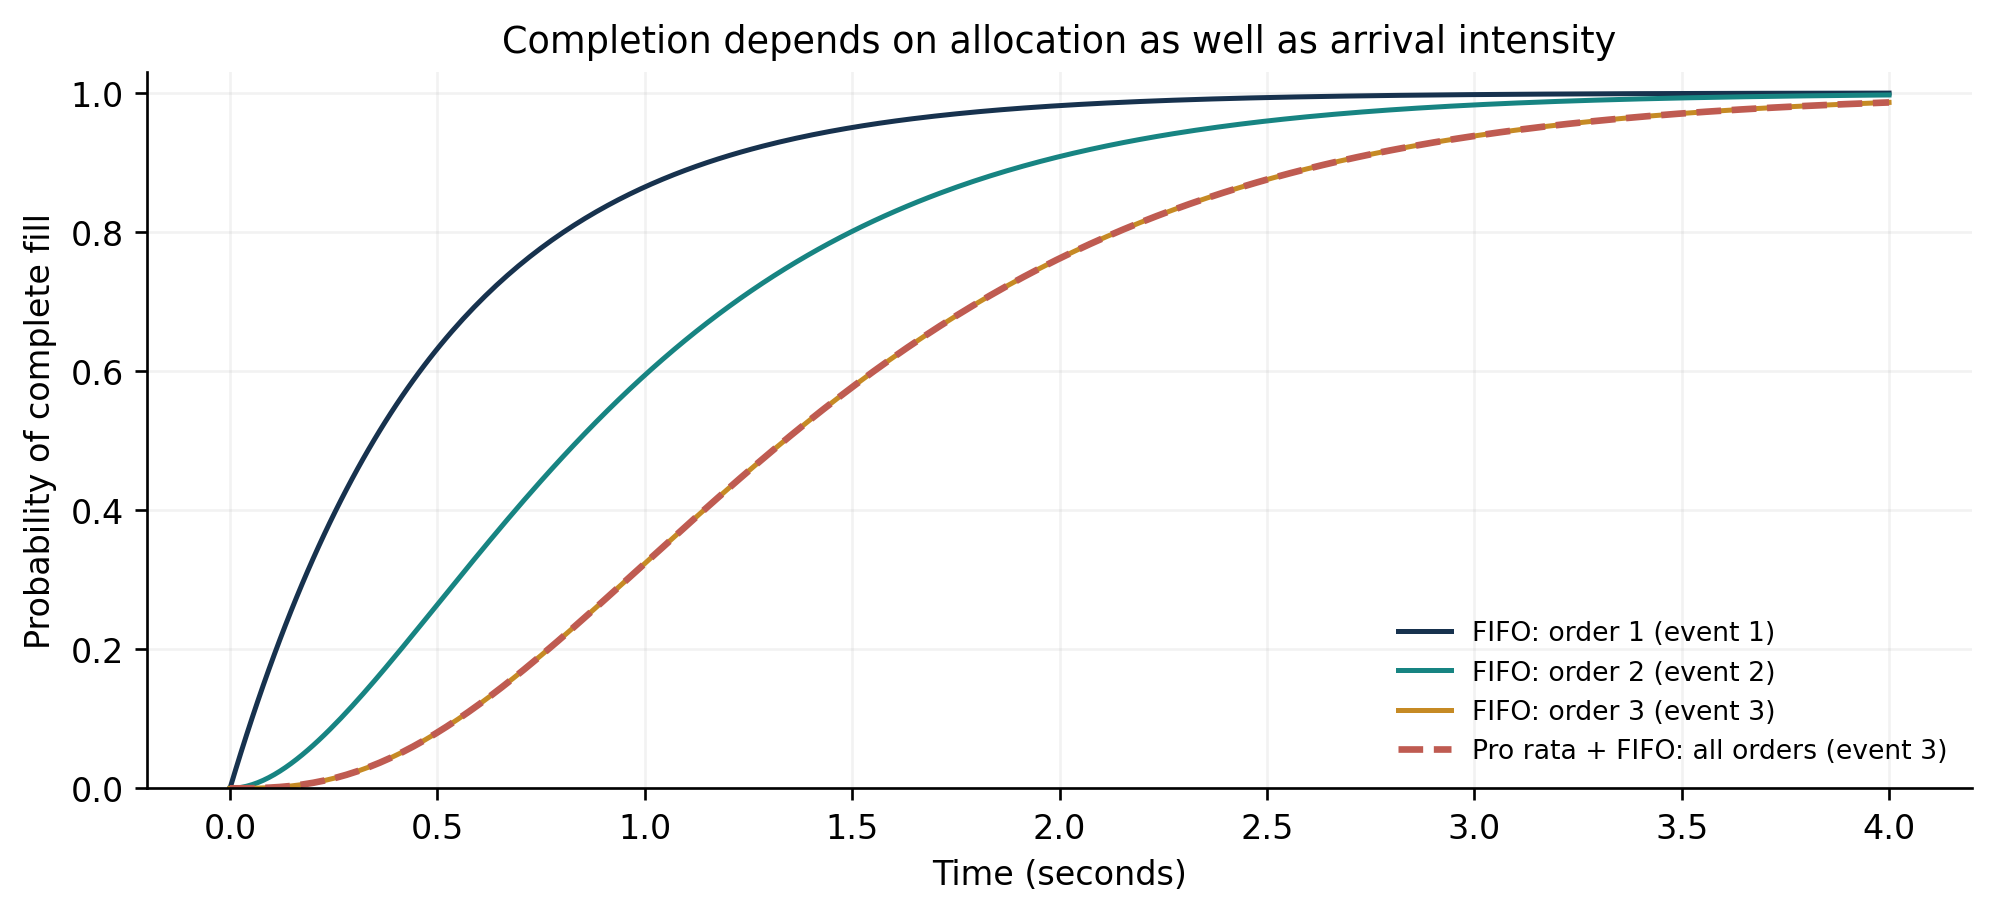
\includegraphics[width=.92\textwidth]{figures/04_completion.png}
\caption{Exact complete-fill distributions in the fixed-batch arrival model. The dashed curve coincides with the third FIFO curve because both require three arrivals. Arrival intensity is an illustrative assumption rather than an empirical estimate.}
\label{fig:completion}
\end{figure}

\subsection{Stochastic state and filtering}

A stochastic model can assign state-dependent intensities $\lambda_e(x)$ to events and generator
\begin{equation}
 (\mathcal Gf)(x)=\sum_e\lambda_e(x)[f(T_e x)-f(x)].
\end{equation}
Deterministic matching and random event arrivals then coexist without making the matching rule itself random. Price controls, cancellations, and replenishment require additional transitions. Queue depletion need not have an Erlang law under those extensions.

If the complete modeled state is Markov with transition matrix $P$ and observations are deterministic, a finite-state belief $\beta_n(x)$ updates through
\begin{equation}
 \beta_{n+1}(x')=
 \frac{\ind\{\Pi(x')=Y_{n+1}\}\sum_x\beta_n(x)P(x,x')}
 {\sum_{u:\Pi(u)=Y_{n+1}}\sum_x\beta_n(x)P(x,u)},
\label{eq:filter}
\end{equation}
when the denominator is positive. This expresses the difference between reconstructing observed messages and inferring unobserved state. A forecast of execution should condition on what was available at the decision time, not on subsequently repaired or future market data.

\section{Opening, reopening, and market boundaries}
\label{sec:opening}

An opening calculation acts on a collection of accumulated eligible orders. It does not have the same event sequence as a stream of continuous aggressors. Nor does a futures market have a universal cash-equity-style closing auction. Opening, session termination, daily settlement, and final expiry must each have their own transition.

\subsection{Eligible quantities and candidate prices}

Fix a finite candidate grid $\mathcal P$ and a snapshot of auction-eligible simple orders. Define
\begin{equation}
 B(p)=\sum_{i\in\mathcal B}q_i\ind\{L_i\ge p\},\qquad
 S(p)=\sum_{i\in\mathcal S}q_i\ind\{L_i\le p\}.
\end{equation}
Under complete one-for-one compatibility,
\begin{equation}
 V(p)=\min\{B(p),S(p)\},\qquad I(p)=B(p)-S(p).
\label{eq:auction}
\end{equation}
The function $B$ is nonincreasing, $S$ is nondecreasing, and $I$ is nonincreasing. An executable opening can contain a crossed book during accumulation because continuous matching is not active in that phase. The same crossed ledger would not be an ordinary stable continuous book.

\begin{proposition}[Auction capacity under full compatibility]
At a fixed $p$, the maximum feasible match quantity is $V(p)$.
\end{proposition}
\begin{proof}
Every trade consumes one eligible contract on each side, giving the upper bound $\min(B,S)$. Pair contracts from the two sides until the smaller side is exhausted. Full compatibility makes every pair admissible, so the bound is attained.
\end{proof}

Account restrictions, minimum quantities, ratio instruments, and other incompatibilities can invalidate this construction. In such cases $V(p)$ should be defined through feasible matching rather than assumed equal to a minimum of totals.

\subsection{CME opening-price branches}

CME's IOP documentation begins with maximum matching quantity. Its rules and worked applications then distinguish imbalance and reference-price cases: minimum unmatched quantity, upward selection for buy-side pressure, downward selection for sell-side pressure, and proximity to prior settlement for a balanced interval \citep{CMEIOPRules,CMEIOPExamples}. We implement the following documented simple-order cases, preserving any unresolved tie as a set rather than inventing a final preference.

Let $\mathcal P_0=\argmax_pV(p)$. If it is a singleton, the primary criterion suffices. For multiple candidates, the examples establish selection of a unique minimum of $|I(p)|$ when one exists, including a zero-versus-nonzero tie in volume. When the maximum-volume candidates all have positive imbalance, choose the highest such price; when all have negative imbalance, choose the lowest. When all are balanced, choose the candidate nearest prior settlement; equal distances remain set-valued here. A remaining two-sided exact tie requires further product and operational treatment beyond these examples.

These branches are compatible with the monotonicity of $I$. On an all-positive candidate set, the highest price has the smallest imbalance; on an all-negative set, the lowest price does. This observation explains the direction of the pressure rule without assuming that every tie is resolved by a generic reference-distance minimization.

\begin{table}[htbp]
\centering\small
\begin{tabular}{@{}lrrrr@{}}
\toprule
Candidate price & $B(p)$ & $S(p)$ & $V(p)$ & $I(p)$\\
\midrule
100 & 15 & 4 & 4 & 11\\
101 & 15 & 9 & 9 & 6\\
102 & 10 & 12 & 10 & $-2$\\
103 & 6 & 12 & 6 & $-6$\\
\bottomrule
\end{tabular}
\caption{A synthetic opening ledger. Buy limits are $103:6$, $102:4$, $101:5$; sell limits are $100:4$, $101:5$, $102:3$. Notation $p:q$ denotes price and contracts.}
\label{tab:opening}
\end{table}

The unique price in Table~\ref{tab:opening} is 102. With a declared price-time allocation on both sides, the two highest-priced buys fill six and four contracts. The sells fill four at limit 100, five at limit 101, and one at limit 102. All ten pairs execute at the selected opening price 102; their limits are eligibility conditions rather than distinct execution prices.

\begin{figure}[htbp]
\centering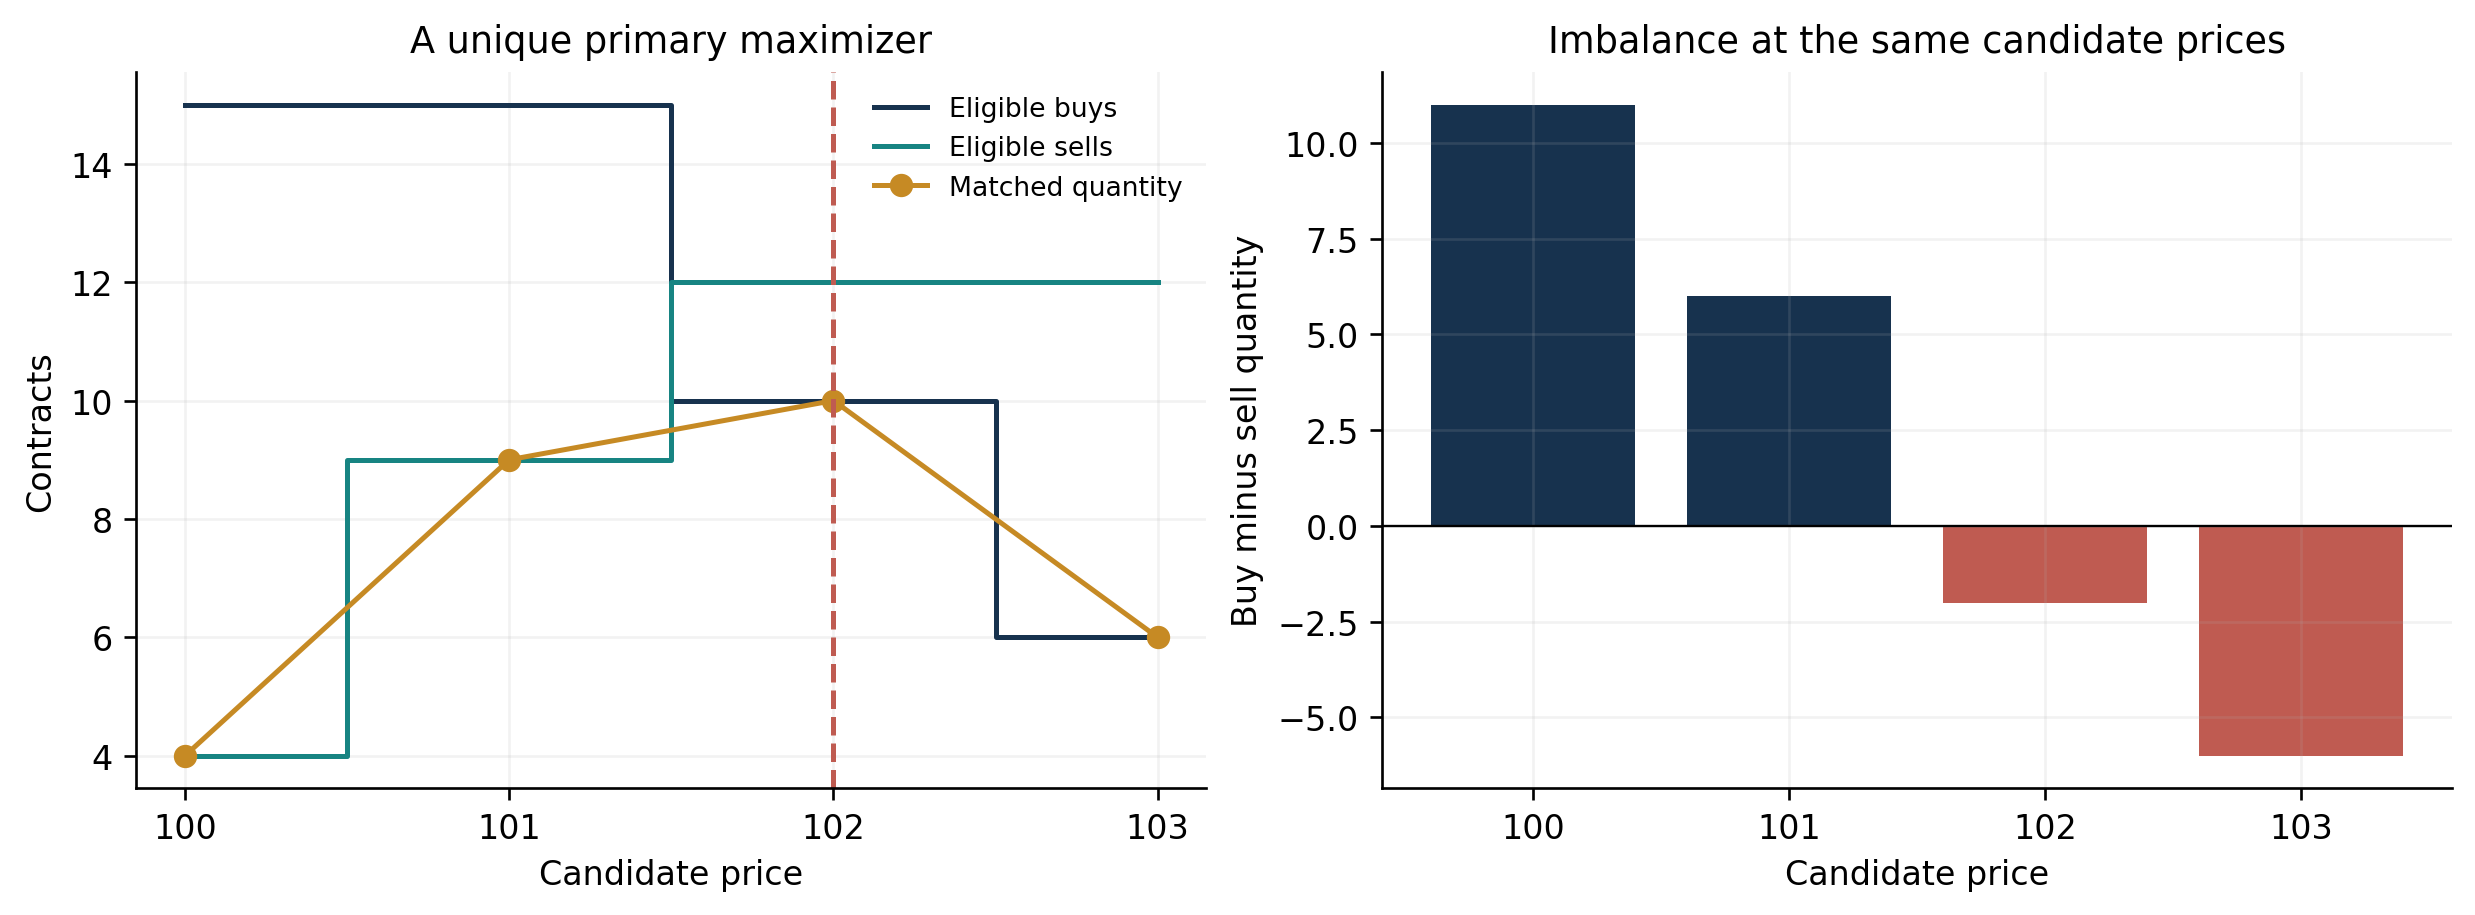
\includegraphics[width=\textwidth]{figures/05_opening.png}
\caption{The quantity and imbalance calculations for Table~\ref{tab:opening}. Price 102 has the largest match quantity despite a sell imbalance. Maximizing volume and setting imbalance to zero are different objectives.}
\label{fig:opening}
\end{figure}

\begin{table}[htbp]
\centering\small
\begin{tabularx}{\textwidth}{@{}lXXXl@{}}
\toprule
Case & Buy orders & Sell orders & Maximizing prices & IOP\\
\midrule
Buy pressure & $103:6$ & $101:4$ & $101,102,103$ & 103\\
Sell pressure & $103:4$ & $101:6$ & $101,102,103$ & 101\\
Balanced & $103:4$ & $101:4$ & $101,102,103$ & 102\\
Opposite signs & $102:4,101:2$ & $101:4,102:3$ & $101,102$ & 101\\
Zero and positive & $102:4,101:2$ & $101:4$ & $101,102$ & 102\\
\bottomrule
\end{tabularx}
\caption{Five synthetic tie cases, with reference settlement 102. The opposite-sign case has imbalances $2$ and $-3$; the last case has imbalances $2$ and $0$. Candidate prices are the listed integer ticks.}
\label{tab:ties}
\end{table}

Opening allocation must be specified separately from opening-price selection. For example, CME's SOFR documentation describes price-time opening treatment, with TOP matching beginning in continuous trading and implied interest unavailable in pre-open \citep{CMEMatching}. One should not apply a continuous-session proportional allocator automatically to an opening ledger.

\subsection{Stop election as a finite activation process}

The IOP rules describe recalculation when an indicative price elects stop orders, using their limit-price quantities until no additional stops are elected \citep{CMEIOPRules}. An abstract implementation starts from an active set $E_0$, calculates $p(E_0)$, and repeatedly applies
\begin{equation}
 E_{k+1}=E_k\cup\{i:\text{stop }i\text{ is elected by }p(E_k)\}.
\end{equation}

\begin{proposition}[Finite activation closure]
If there are $N$ initially inactive stops, no new orders arrive during the calculation, and an elected stop remains active, the iteration has at most $N$ strict enlargements before reaching a fixed active set.
\end{proposition}
\begin{proof}
The active sets form an increasing chain of subsets of a finite set. Every strict enlargement adds at least one previously inactive stop. There can be at most $N$ such additions.
\end{proof}

The proof does not establish that indicative prices are monotone. It also does not resolve an ambiguous price-selection branch. A reproducible algorithm needs both a fixed activation convention and a price-selection rule defined for its inputs. The supplied numerical opening examples contain no stops, so they do not depend on a hidden convention for unresolved ties.

\subsection{A primary-volume stability margin}

\begin{proposition}[A sharp functional gap bound]\label{prop:gap}
Suppose $V$ on a finite grid has a unique maximizer $p^*$ and gap
\begin{equation}
 g=V(p^*)-\max_{p\ne p^*}V(p)>0.
\end{equation}
If $\|\widehat V-V\|_\infty\le\varepsilon$ and $g>2\varepsilon$, then $p^*$ remains the unique primary maximizer. The constant two is sharp over arbitrary bounded perturbations of $V$.
\end{proposition}
\begin{proof}
For any competitor $p$, $\widehat V(p^*)-\widehat V(p)\ge g-2\varepsilon>0$. For sharpness choose a runner-up $p_2$, lower $V(p^*)$ by $\varepsilon$, and raise $V(p_2)$ by $\varepsilon$. The resulting difference is $g-2\varepsilon$, giving a tie at equality and reversal below it.
\end{proof}

If both cumulative sides change by at most $\delta$ uniformly, then $|\min(\widehat B,\widehat S)-\min(B,S)|\le\delta$, so the same sufficient bound applies with $\varepsilon=\delta$. The sharpness construction is a statement about the class of volume functions; it need not be realizable by a single order amendment in a constrained book. In Table~\ref{tab:opening}, the volume gap is only one contract, illustrating the limited protection afforded by the primary criterion alone.

\subsection{Closing a session and controlling prices}

For a phase boundary, let $\mathcal P(\phi)$ be the permitted price set and $\mathcal E(\phi)$ the permitted events. A resting order outside a new permitted range is not automatically a trade. An execution transition must also have a compatible counterparty and a matching phase. Clipping a simulated transaction price to a limit while keeping its quantity is therefore generally incorrect.

In the ES rulebook, trading-day termination is distinct from the afternoon reference interval used for price controls; the ordinary session extends beyond that interval \citep{CME358}. Our model treats session close as a phase transition with order-lifetime processing. Section~\ref{sec:settlement} separately treats the daily settlement statistic. Neither operation is assumed to be a uniform-price closing auction.
\FloatBarrier

\section{Daily settlement and exact cash accounting}
\label{sec:settlement}

\subsection{The settlement price is a rule-defined statistic}

CME publishes product-specific daily and final settlement procedures, including exceptional determination when the ordinary calculation is unavailable or unrepresentative \citep{CMESettlements}. A last traded price, a midquote, a daily settlement, and a final settlement can be different numbers.

For the ordinary lead ES month, the consulted procedure uses the Globex trade VWAP in the 14:59:30--15:00:00 Central Time window, rounded to 0.25 index point. Its no-trade branches use other information, and other contract months have their own procedures \citep{CMESettleES}. Accordingly, the following formula is conditional on a nonempty eligible trade set in that branch:
\begin{equation}
 \overline p_W=\frac{\sum_{k\in W}v_kp_k}{\sum_{k\in W}v_k},
 \qquad s=\mathcal R_{\tau}(\overline p_W),\qquad \tau=0.25.
\label{eq:vwap}
\end{equation}
The operator $\mathcal R_\tau$ means rounding under the applicable convention. Our examples avoid an exact midpoint tie. Setting a missing VWAP to zero would create a fictional settlement; the required branch is instead a different statistic.

\begin{proposition}[One added trade and a rounding boundary]
If a window with positive total quantity $N$ and VWAP $\overline p$ receives an additional eligible trade of size $r$ at $p$, then
\begin{equation}
 \overline p'=\overline p+\frac{r}{N+r}(p-\overline p).
\label{eq:vwapshift}
\end{equation}
If the original VWAP is strictly within a rounding cell, perturbations smaller than its distance to the nearest cell boundary leave the rounded settlement unchanged.
\end{proposition}
\begin{proof}
Subtract $\overline p$ from $(N\overline p+rp)/(N+r)$. The rounding claim follows because the perturbed value remains in the same cell.
\end{proof}

For synthetic window trades $(6000,4)$, $(6000.25,2)$, and $(6000.50,4)$, the VWAP and rounded settlement are both 6000.25. Adding three contracts at 6001.00 produces a VWAP of $6000.423076\ldots$ and rounded settlement 6000.50. The statistic moves one tick. For an unchanged ten-contract ES position, that mark difference is \$125; it is not a statement about the added trader's profit, execution costs, or ability to influence a live benchmark.

\subsection{Round value first, then difference}

For the normal futures convention described in CME's money-calculation specification, define the one-contract value
\begin{equation}
 \nu_j(p)=\mathcal R_{c_j}(m_jp),
\label{eq:moneyvalue}
\end{equation}
where $c_j$ is the settlement currency's precision. A mark from $p$ to $s$ for signed quantity $n$ is $n[\nu_j(s)-\nu_j(p)]$. This order of operations preserves lot-splitting and intermediate-mark consistency. The document distinguishes normal rounding from special notional and inverse conventions \citep{CMEMoney}. The results below concern the normal convention, with a fixed deterministic value map.

For USD, decimal half-way values are rounded away from zero in the cited normal convention. Thus a synthetic one-contract value of 1.005 becomes 1.01, while $-1.005$ becomes $-1.01$. Binary floating-point rounding and banker's rounding should not silently replace that convention. In the ES ledger all relevant one-contract values are already exact cents.

\subsection{A changing-position identity}

For one future, let $z_{t-1}$ be the position carried into clearing cycle $t$, let $s_{t-1},s_t$ be its previous and current settlement prices, and let trades in the cycle have signed quantities $n_{tk}$ and prices $p_{tk}$. Positive quantity means a purchase. Then
\begin{align}
 z_t&=z_{t-1}+\sum_kn_{tk},\\
 \mathrm{VM}_t&=z_{t-1}[\nu(s_t)-\nu(s_{t-1})]
       +\sum_kn_{tk}[\nu(s_t)-\nu(p_{tk})].
\label{eq:vm}
\end{align}
For multiple contracts, sum these expressions by contract and currency. FX conversion, if required for reporting, is a separate operation.

\begin{theorem}[Settlement telescoping with trades]\label{thm:telescoping}
For a fixed normal money-value map and the position recursion above,
\begin{equation}
 \sum_{t=1}^T\mathrm{VM}_t
 =z_T\nu(s_T)-z_0\nu(s_0)
       -\sum_{t=1}^T\sum_kn_{tk}\nu(p_{tk}).
\label{eq:telescoping}
\end{equation}
Consequently, if initial and final positions are zero, total variation equals signed sale value minus signed purchase value. Subdividing a trade at the same price, or inserting intermediate marking points without changing the value map or trades, leaves the total unchanged.
\end{theorem}
\begin{proof}
Substitute $z_t=z_{t-1}+\sum_kn_{tk}$ into \eqref{eq:vm} to obtain
\[
 \mathrm{VM}_t=z_t\nu(s_t)-z_{t-1}\nu(s_{t-1})
                 -\sum_kn_{tk}\nu(p_{tk}).
\]
Summing cancels adjacent position-value terms. Trade splitting preserves the sum because quantities enter linearly. Intermediate marks cancel by the same telescoping identity.
\end{proof}

The final sentence concerns total cash transfers before financing costs. It does not say that cash can arrive after its payment deadline. It also assumes a fixed contract-value convention; corporate actions, contract conversions, daily adjustments, currency conversion, or other exceptional rules would require additional ledger terms.

For a held constant position $z$, \eqref{eq:telescoping} reduces to $z[\nu(s_T)-\nu(s_0)]$. If the position changes, simply multiplying the final position by the total price change is wrong. Trades within a clearing cycle can have realized economic effects even when the final position is zero.

\subsection{Cash, posted collateral, and equity}

Let $b_t$ be free cash and $P_t$ posted cash collateral, measured immediately after cycle $t$. Let $D_t$ be net new external funding, $f_t$ fees, and $\Delta P_t=P_t-P_{t-1}$. A single-currency accounting identity is
\begin{equation}
 b_t=b_{t-1}+\mathrm{VM}_t+D_t-f_t-\Delta P_t.
\label{eq:cash}
\end{equation}
Adding posted collateral yields
\begin{equation}
 b_t+P_t=b_{t-1}+P_{t-1}+\mathrm{VM}_t+D_t-f_t.
\end{equation}
Posting margin reduces free cash but does not itself create a trading loss. Releasing margin increases free cash but does not create trading profit. Noncash collateral requires separate valuation and transfer accounts rather than insertion into $b_t$ as immediately spendable money.

The clearing-cycle index is intentionally more general than a calendar-day index. CME's safeguards description identifies regular intraday and end-of-day processes for futures and options \citep{CMESafeguards}. Customer calls can also depend on the clearing firm's own arrangements. The three-day example in Section~\ref{sec:ledger} aggregates to one displayed cycle per day for exposition.
\FloatBarrier

\section{The geometry of portfolio risk and margin}
\label{sec:margin}

\subsection{What the public SPAN 2 description establishes}

CME's public SPAN 2 methodology separates historical risk, stress risk, liquidity, and concentration. It describes a weighted historical/stress market-risk component and additional closeout and concentration charges. Historical scenario generation includes volatility and correlation treatment and option-volatility risk factors \citep{CMESPAN2}. Its risk overview also discusses SPAN and SPAN 2 together \citep{CMERisk}. These sources do not justify assuming that every product has migrated, that one parameter set applies to every portfolio, or that a maximum of six losses is a production margin calculation.

We therefore define an independent educational functional. Its purpose is to make the geometry and the distinction between price risk and funding explicit. None of its numerical charges below is quoted as a CME requirement.

\subsection{A declared finite-scenario functional}

Let $z\in\R^d$ be holdings and $g_s\in\R^d$ the per-contract monetary loss vector in scenario $s=1,\ldots,S$. A scenario can contain full repricing of each instrument. Even if an option's price is nonlinear in its market risk factors, its portfolio contribution remains linear in the number of identical options held when per-instrument scenario values are fixed.

Define
\begin{equation}
 R(z)=\max\{0,g_1^\top z,\ldots,g_S^\top z\}.
\label{eq:scenario}
\end{equation}
The zero scenario makes the risk charge nonnegative. Writing $G=\conv\{0,g_1,\ldots,g_S\}$, $R$ is the support function of $G$: $R(z)=\max_{g\in G}g^\top z$.

\begin{proposition}[Convexity, offsets, and sensitivity]\label{prop:risk}
The functional $R$ is convex, positively homogeneous, and subadditive. For any norm and its dual,
\begin{equation}
 |R(z)-R(z')|\le\max_s\|g_s\|_*\,\|z-z'\|.
\end{equation}
Every active loss vector is a subgradient. If one vector is uniquely active in a neighborhood, it is the gradient there. If the scenario set is symmetric and spans $\R^d$, $R$ is a norm; otherwise it may fail symmetry or positive definiteness.
\end{proposition}
\begin{proof}
A maximum of linear functions is convex and positively homogeneous for nonnegative scalars. For each $g\in G$, $g^\top(z+z')\le R(z)+R(z')$, proving subadditivity after maximization. If $g$ maximizes at $z$, then $R(z)-R(z')\le g^\top(z-z')\le\|g\|_*\|z-z'\|$; reverse the arguments for the absolute bound. An active $g$ satisfies $R(u)\ge g^\top u=R(z)+g^\top(u-z)$, giving the subgradient property. Symmetry gives $R(-z)=R(z)$, and spanning prevents $R(z)=0$ for nonzero $z$ when both signs of every vector are present.
\end{proof}

Subadditivity permits a portfolio risk charge below the sum of standalone charges. It does not imply that changing any position toward zero reduces portfolio risk: the position may be a hedge for another position.

For explicit liquidity and concentration illustrations let $G_1(z)=\sum_j|z_j|$ and
\begin{equation}
 M(z)=R(z)+aG_1(z)+b\pos{G_1(z)-H}^2,
 \qquad a,b,H\ge0.
\label{eq:margin}
\end{equation}
Both additions are convex, so $\{z:M(z)\le c\}$ is convex. The quadratic addition removes positive homogeneity and can produce increasing marginal charges for large portfolios. This is a chosen mathematical model, not a derivation of CME's production add-on formulas. Risk parameters are fixed throughout this convexity statement; if they change with time or the portfolio, the function must be reassessed.

\subsection{A hedge-removal counterexample}

Take two futures with the six loss vectors in Table~\ref{tab:risk}. They correspond to a \$1,000 value factor and six declared two-leg price shocks. The risk is
\begin{equation}
 R(z_1,z_2)=\max\{2000|z_1+z_2|,
                  1000|z_1-z_2|,1000|3z_1+z_2|\}.
\end{equation}

\begin{table}[htbp]
\centering\small
\begin{tabular}{@{}lrrrr@{}}
\toprule
Scenario & $g_{s1}$ & $g_{s2}$ & Loss at $(5,-5)$ & Loss at $(5,-3)$\\
\midrule
1 & 2,000 & 2,000 & 0 & 4,000\\
2 & $-2,000$ & $-2,000$ & 0 & $-4,000$\\
3 & 1,000 & $-1,000$ & 10,000 & 8,000\\
4 & $-1,000$ & 1,000 & $-10,000$ & $-8,000$\\
5 & 3,000 & 1,000 & 10,000 & 12,000\\
6 & $-3,000$ & $-1,000$ & $-10,000$ & $-12,000$\\
\bottomrule
\end{tabular}
\caption{Synthetic per-contract and portfolio losses in dollars. Positive numbers are losses and negative numbers are gains. The zero scenario in \eqref{eq:scenario} is implicit.}
\label{tab:risk}
\end{table}

At $(5,-5)$, $R=\$10{,}000$, compared with $R(5,0)+R(0,-5)=\$25{,}000$. With $a=100$, $b=50$, $H=8$, total illustrative margin is
\begin{equation}
 M(5,-5)=10{,}000+1{,}000+200=\$11{,}200.
\end{equation}
Closing two short contracts leaves $(5,-3)$. Gross contracts fall from ten to eight, but
\begin{equation}
 M(5,-3)=12{,}000+800+0=\$12{,}800.
\end{equation}
The partial liquidation removes a hedge against scenario 5. A rule that assumes every position reduction releases collateral would understate the new requirement by \$1,600 relative to the old one, even before execution costs.

\begin{figure}[htbp]
\centering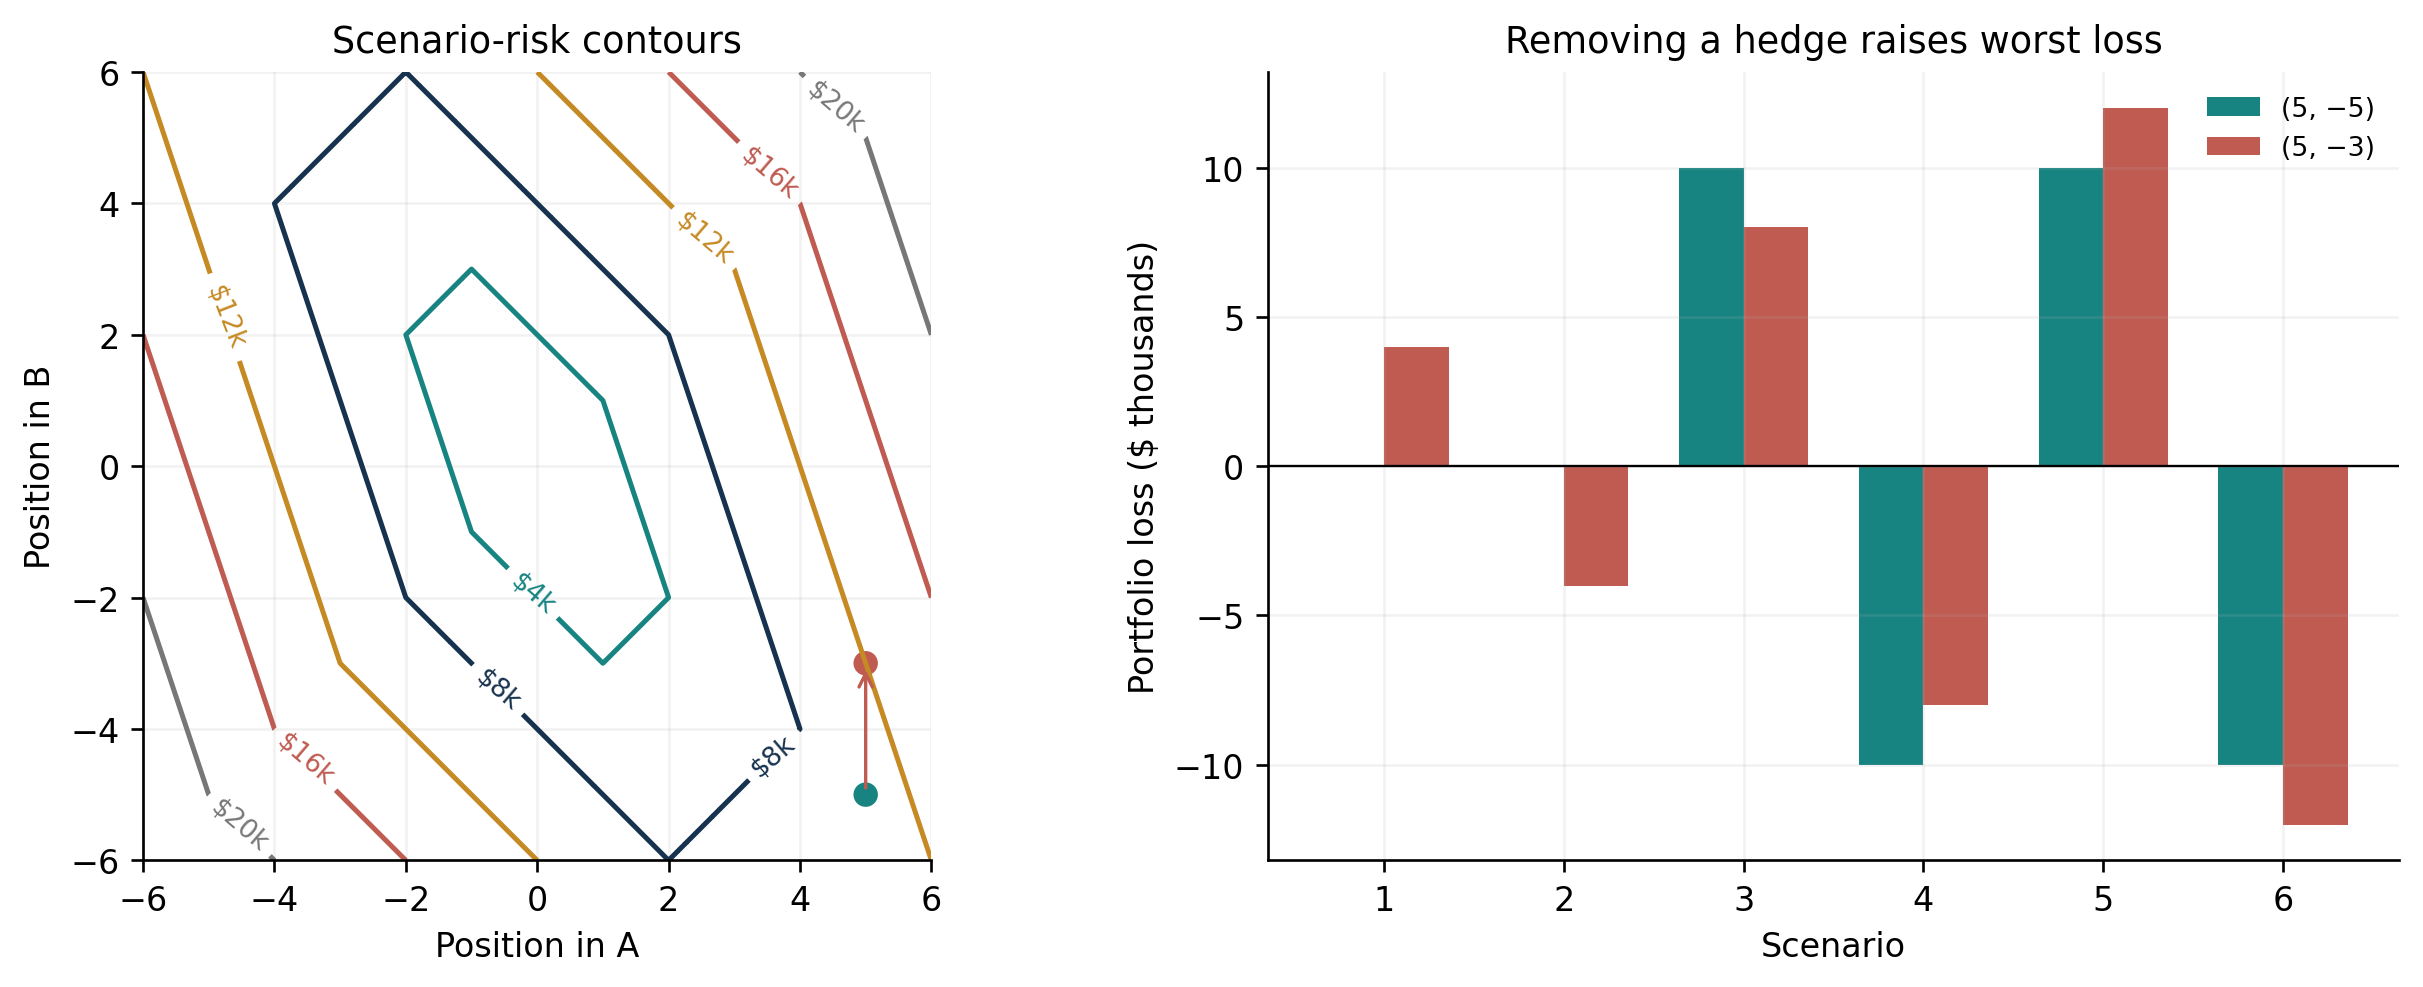
\includegraphics[width=\textwidth]{figures/07_margin.png}
\caption{Risk contours and scenario losses for the declared model. Moving from $(5,-5)$ to $(5,-3)$ crosses toward a larger worst-loss contour. Convexity in portfolio space is compatible with increased risk after removing one hedge leg.}
\label{fig:margin}
\end{figure}

\subsection{Historical quantiles and expected shortfall}

A historical value-at-risk calculation is a quantile, not generally a maximum. For scenario losses $L_s(z)=g_s^\top z$ with probabilities $\pi_s$, define
\begin{equation}
 \VaR_\alpha(z)=\inf\{a:\sum_{s:L_s(z)\le a}\pi_s\ge\alpha\}.
\end{equation}
A convex alternative, using the standard variational representation of \citet{Rockafellar2000}, is
\begin{equation}
 \ES_\alpha(z)=\min_{a\in\R}
 \left[a+\frac{1}{1-\alpha}\sum_s\pi_s\pos{L_s(z)-a}\right].
\label{eq:es}
\end{equation}
The representation handles discrete probability mass at the quantile by taking the required fraction of that mass. It should not be replaced with an unqualified conditional average over losses strictly above the quantile. For equal probabilities and a tail containing an integer number of observations, it is the average of that many largest losses. In Table~\ref{tab:risk}, at $(5,-3)$ and $\alpha=2/3$, the six-scenario VaR is \$4,000 while expected shortfall is $(8000+12000)/2=\$10,000$. The worst loss is \$12,000.

Convexity cannot be inferred from the word ``VaR.'' To see this directly, let two disjoint events each have probability 0.04. One position loses 100 only on the first event and a second loses 100 only on the second. Each has 95\% VaR zero, but their combined loss has 95\% VaR 100. The midpoint portfolio has VaR 50, violating convexity relative to the two individual positions. Hence Proposition~\ref{prop:risk} is a property of its declared risk functional, not a theorem about any production historical-quantile margin system.

\subsection{Which sensitivity is being measured?}

At least three sensitivities should be separated: a portfolio changes with risk parameters fixed; market conditions change and the risk parameters are recomputed; or available collateral changes while the required margin remains fixed. A large variation payment can coincide with any of these. The first sensitivity is described by $R$ and $M$ above. The second needs a model for $\theta_t$. The third is a resource-feasibility question, considered next.
\FloatBarrier

\section{Collateral feasibility and the timing of funding}
\label{sec:funding}

\subsection{A scalar balance is not a collateral allocation}

CME distinguishes collateral accepted from clearing members from the criteria applicable to account holders through their clearing firms. Public schedules identify eligible assets, haircuts, currency treatment, and concentration limits \citep{CMECollateral,CMEAcceptable}. Assets belonging to different legal accounts cannot be combined merely because a researcher can add their market values.

For a fixed legal account and deadline, let asset $i$ have available amount $c_i$. Allocate $x_{ji}\ge0$ of that asset to requirement $j$. One unit provides credit $a_{ji}\ge0$, where zero means ineligible. Then
\begin{equation}
 \sum_jx_{ji}\le c_i\quad\text{for every asset }i,
 \qquad \sum_i a_{ji}x_{ji}\ge d_j\quad\text{for every requirement }j.
\label{eq:collateral}
\end{equation}
The coefficients contain declared valuation and haircut conversions. Additional concentration or issuer constraints would add rows to this program. The same asset cannot be counted in several requirements without consuming capacity.

\begin{proposition}[Weighted collateral feasibility]\label{prop:collateral}
In the fractional allocation model \eqref{eq:collateral}, with finite assets and requirements, $c_i,d_j,a_{ji}\ge0$, feasibility is equivalent to
\begin{equation}
 \sum_j\lambda_jd_j
 \le\sum_ic_i\max_j\{\lambda_ja_{ji}\}
 \qquad\text{for every }\lambda\in\R_+^J.
\label{eq:collateraldual}
\end{equation}
\end{proposition}
\begin{proof}
For any allocation and nonnegative $\lambda$, weighted supplied credit is at most $\sum_ic_i\max_j\lambda_ja_{ji}$, since each unit of asset $i$ can be assigned only once. This proves necessity.

For sufficiency let $C$ be the compact convex set of credit vectors attainable by allocations satisfying the asset capacities. Requirements are feasible precisely when $d\in C-\R_+^J$. This latter set is closed, convex, and downward closed. If $d$ is outside, a strict separating hyperplane exists. Its normal can be chosen nonnegative: a negative component would give an infinite supremum in that coordinate's downward direction. For its normal $\lambda$, the supremum over $C$ is $\sum_ic_i\max_j\lambda_ja_{ji}$, obtained by assigning each asset to a maximizing requirement. Separation contradicts \eqref{eq:collateraldual}.
\end{proof}

This finite-dimensional result is an application of convex separation and linear-programming duality, not a claim about a complete collateral service. Divisibility, absence of additional caps, and time availability are explicit assumptions. Indivisible assets require an integer model; concentration constraints alter the right-hand support calculation.

\begin{example}[Enough value, too little cash]\label{ex:collateral}
An account has \$5,000 cash and \$20,000 of bond market value. In this synthetic model, bonds receive a 10\% haircut against an initial-margin requirement of \$10,800 but cannot meet the current cash variation payment without a separate sale or financing transaction. Total credited resources are \$23,000.

With a \$4,000 variation payment, allocate \$4,000 cash to variation and \$12,000 bond value to initial margin. This leaves \$1,000 cash and \$8,000 unallocated bonds. With a \$6,000 variation payment, total requirements are only \$16,800, below \$23,000, but the allocation is infeasible because cash is short by \$1,000. In \eqref{eq:collateraldual}, choose weight one on the cash requirement and zero on initial margin to certify the failure.
\end{example}

The haircut is illustrative, not a quoted live CME rate. If bonds can be converted to cash before the deadline, that transaction belongs in the model with its own timing, haircut, cost, and availability. Its existence must not be assumed from the bond's market value alone.

\subsection{Minimum funding is a prefix maximum}

Take an ordered sequence of cash events. Let $r_t\ge0$ be actual receipts available at event $t$ and $d_t\ge0$ obligatory payments, including increases in posted cash collateral where applicable. Releases enter receipts. Assume zero interest, no borrowing after inception, and free retention of receipts. With initial free cash $F$,
\begin{equation}
 b_t=F+\sum_{u=1}^t(r_u-d_u).
\end{equation}

\begin{theorem}[Exact minimum initial funding]\label{thm:funding}
The smallest $F\ge0$ for which every payment can be met in the specified event order is
\begin{equation}
 F^*=\max\left\{0,\max_{1\le t\le T}\sum_{u=1}^t(d_u-r_u)\right\}.
\label{eq:funding}
\end{equation}
\end{theorem}
\begin{proof}
Each constraint $b_t\ge0$ requires $F\ge\sum_{u\le t}(d_u-r_u)$. Their maximum is necessary. Setting $F$ to that maximum satisfies every constraint, establishing sufficiency.
\end{proof}

If a debit precedes a receipt within a nominal clearing cycle, they must be separate events in this theorem. Netting their amounts into one simultaneous event would understate the required funding. The formula measures additional \emph{free cash}; collateral already posted at inception is accounted for separately.

\begin{example}[Identical terminal gain, different liquidity demand]\label{ex:funding}
Hold ten ES contracts from settlement 6,000. Compare settlement paths
\[
 A:(6000,5980,6004),\qquad B:(6000,6002,6004).
\]
Path A produces variation payments $-\$10,000,+\$12,000$; path B produces $+\$1,000,+\$1,000$. Both end with a \$2,000 gain. If initial margin is already posted and unchanged, $F_A^*=\$10,000$ and $F_B^*=0$.

If path A also requires \$5,000 additional cash margin at the first cycle, released at the second, its cumulative free-cash changes become $(-15{,}000,+2{,}000)$. Required initial free cash rises to \$15,000. Starting with \$8,000 leaves a \$7,000 shortfall at the first call despite the positive terminal gain.
\end{example}

\begin{figure}[htbp]
\centering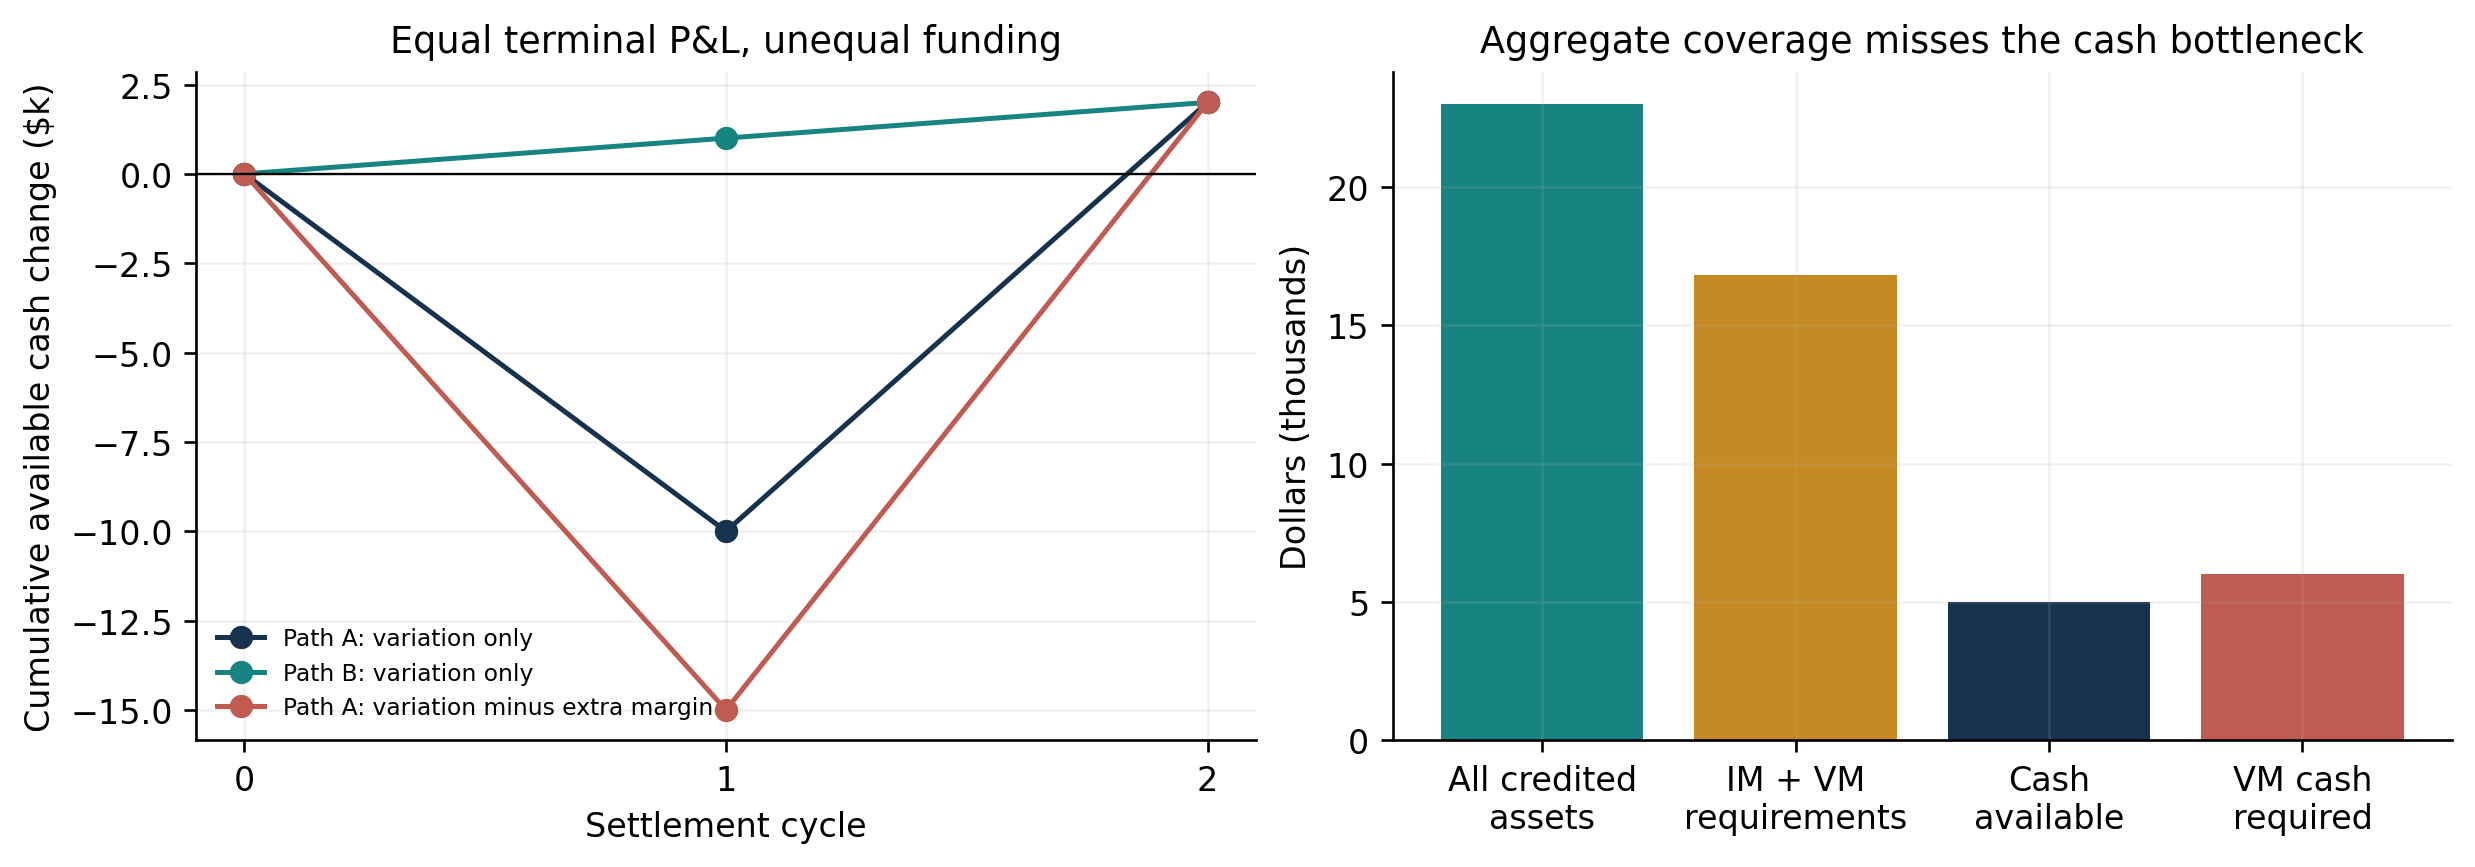
\includegraphics[width=\textwidth]{figures/08_funding.png}
\caption{Two distinct failures of scalar risk summaries. Left: timing changes required funding even with the same final gain. Right: aggregate collateral value cannot replace a cash-eligibility constraint. Parameters are synthetic.}
\label{fig:funding}
\end{figure}

\subsection{Execution under a margin constraint}

Let $u$ be a vector of proposed trades and $z+u$ the resulting positions. A local optimization might trade execution shortfall against a target exposure and a margin charge:
\begin{equation}
 \min_{u\in\mathcal U(X)}
 \left\{\mathrm{IS}(u;X)+\eta M(z+u)
       +\gamma\|z+u-z^{\rm target}\|^2\right\}.
\label{eq:localcontrol}
\end{equation}
The admissible set $\mathcal U(X)$ must enforce integer contracts, available book and recipe capacities, account permissions, price limits, and funding at the relevant deadlines. A favorable marked P\&L is not immediately available cash unless its receipt time is included. A strategy that reduces gross contracts may increase $M$, as Section~\ref{sec:margin} demonstrates.

For a finite-state, finite-action illustration with transition kernel $P_t(x'\mid x,u)$, admissible actions $\mathcal U_t(x)$, and stage cost $c_t$, the continuation value satisfies
\begin{equation}
 J_t(x)=\min_{u\in\mathcal U_t(x)}
 \left[c_t(x,u)+\sum_{x'}P_t(x'\mid x,u)J_{t+1}(x')\right].
\end{equation}
States with no feasible continuation have value $+\infty$. Under partial observation the state for control is a belief such as \eqref{eq:filter}, together with directly known private cash and positions. This equation describes a modeling architecture; no optimal trading policy or empirical transition kernel is estimated here.

The economically relevant feasible set is thus the intersection of execution feasibility, portfolio risk capacity, and deadline-specific funding. Each can bind while the other two appear ample.
\FloatBarrier

\section{Options, final settlement, and delivery}
\label{sec:delivery}

\subsection{An option changes the cash convention}

A premium-style option purchase has a premium cash outflow, unlike entry into an ordinary future. The normal premium calculation uses the rounded monetary premium per option multiplied by signed quantity. Futures-style options have different premium and variation treatment; those conventions must not be merged \citep{CMEMoney}.

Let a premium-style call have strike $K$, one underlying future per option, and value factor $m$. Its idealized terminal intrinsic value is $m(F-K)_+$ per option. That value does not specify the operational form of settlement. For an option that exercises into a future, a long call produces a long underlying future at strike, and a long put produces a short future at strike. Their assigned counterparties receive the opposite futures positions. CME's ES option chapter defines an option on one ES future and distinguishes series with different exercise characteristics \citep{CME358A}. The appropriate series must be part of the contract state.

For accepted exercises and assignments, a compact position map is
\begin{equation}
 \Delta z^{\rm fut}=n_{LC}-n_{SC}-n_{LP}+n_{SP},
\end{equation}
where the four nonnegative counts denote long calls exercised, short calls assigned, long puts exercised, and short puts assigned. Each resulting future has its own strike transaction. Different strikes must be retained separately in the variation calculation.

\begin{example}[Exercise is an entry into the futures ledger]\label{ex:option}
Buy two premium-style calls on ES, each at a premium of 18.00 points and strike 6,000. The premium paid is $2\cdot50\cdot18=\$1,800$. Suppose both are validly exercised, each creating a long ES future at 6,000, and the relevant subsequent futures mark is 6,030. The new futures produce
\begin{equation}
 2[\nu(6030)-\nu(6000)]=\$3,000
\end{equation}
of variation. Net cash through that mark, before margin, financing, and fees, is \$1,200. There are still two futures positions unless they are closed or finally settled. Closing both at exactly 6,030 adds no further gain relative to that mark.
\end{example}

Adding both a separate \$3,000 intrinsic-value payment and the \$3,000 futures variation would double count the same economic value in this exercise convention. Conversely, recording only the option's disappearance would omit the new futures positions and their margin and expiry obligations.

Option exercise may change portfolio risk sharply. A model that approximates the option before exercise by a fractional delta must still convert an actual exercised contract into its specified integer futures position. Risk-factor nonlinearity and contract-count discreteness are different sources of nonlinearity.

\subsection{Cash-settled futures at expiry}

For a cash-settled future, final settlement closes the remaining valuation obligation through the contract's final-price rule. ES uses a special opening quotation of its underlying index, subject to the rulebook's exceptions \citep{CME358}. It is not simply the last futures trade or the previous afternoon's daily settlement.

For a position $z$ already marked to $s_{T-1}$, the final variation is
\begin{equation}
 z[\nu(s_T^{\rm final})-\nu(s_{T-1})].
\end{equation}
The settlement transition then removes the expired position. The ledger should preserve the sequence: determine the final reference, calculate the remaining variation, and discharge the contract. Removing the position before calculating the final variation would lose the last cash flow.

\subsection{Physical delivery introduces a second resource system}

The NYMEX CL contract specifies nominal units of 1,000 barrels and physical delivery at Cushing under the contract's grade, location, and procedural requirements \citep{NYMEX200}. A financial position near expiry therefore interacts with physical capacity, documentation, and payment resources. For a simplified nominal-unit planning model, $n$ long contracts require capacity to receive $1000n$ barrels and fund the invoice. A short position requires deliverable supply or another contractually valid resolution. Actual permitted tolerances and procedures remain governed by the rulebook.

A physical planning problem can be written
\begin{equation}
 Dv\le h,\qquad Ev=r(z),
\end{equation}
where $v$ allocates eligible physical resources, $h$ records capacities, and $r(z)$ records obligations generated by the expiring position. The structure resembles implied-liquidity constraints, but the resources, deadlines, and legal requirements are different. A warehouse balance, a pipeline right, and a cash balance should not be collapsed into one scalar ``liquidity'' variable.

The futures position can be financially marked before delivery completes. The delivery invoice is an additional asset-for-cash transaction, not a second payment of cumulative futures P\&L. A combined futures-and-physical ledger must include both and retain their signs.

\subsection{Treasury conversion factors and delivery choice}

For the CBOT Treasury note contract in Chapter 19, the delivery invoice uses the specified futures settlement price $F$, a conversion factor $c_k$ for deliverable $k$, and accrued interest $a_k$. Per contract,
\begin{equation}
 \mathrm{Invoice}_k(F)=\mathcal R_{0.01}(1000Fc_k)+a_k.
\label{eq:invoice}
\end{equation}
The source specifies the relevant notice-day price and the deliverable basket \citep{CBOT19}. Our example fixes a single permissible delivery date and compares synthetic eligible securities; it does not identify a currently cheapest actual Treasury.

Let $P_k$ be the clean acquisition price in points on that date, and assume acquisition and delivery use the same accrued interest. Ignoring cent rounding temporarily, acquisition cost minus invoice is
\begin{equation}
 N_k(F)=1000(P_k-Fc_k).
\label{eq:ctd}
\end{equation}
Accrued interest cancels in this fixed-date comparison. Financing, coupons received during a holding period, repo terms, transaction costs, and timing choices would change the comparison if acquisition occurs earlier.

\begin{proposition}[A delivery envelope]
On a fixed finite deliverable set with $P_k,c_k$ held constant, $N(F)=\min_kN_k(F)$ is continuous, piecewise affine, and concave. A switch between two distinct conversion factors can occur only at
\begin{equation}
 F_{ij}=\frac{P_i-P_j}{c_i-c_j}.
\end{equation}
Not every pairwise intersection lies on the lower envelope.
\end{proposition}
\begin{proof}
The minimum of finitely many affine functions is a continuous concave piecewise-affine function. A pair can exchange order only where its two affine values agree, giving the stated expression. Other deliverables may have smaller values at that point.
\end{proof}

\begin{table}[htbp]
\centering\small
\begin{tabular}{@{}lrrrrr@{}}
\toprule
Deliverable & Clean price & Factor & Accrued & Invoice at 110 & Net cost\\
\midrule
A & 99.00 & 0.9000 & \$600 & \$99,600 & \$0\\
B & 101.00 & 0.9200 & \$800 & \$102,000 & $-\$200$\\
C & 98.00 & 0.8800 & \$500 & \$97,300 & \$1,200\\
\bottomrule
\end{tabular}
\caption{A fixed-date synthetic delivery comparison. Net cost is acquisition including accrued interest minus invoice. B minimizes that cost at $F=110$; A and B cross at $F=100$.}
\label{tab:delivery}
\end{table}

The negative delivery cost for B is a comparison at the given invoice price. Total economics also include the short futures position's entry and variation history. It is not by itself a trading-profit claim. The envelope describes the seller's delivery choice conditional on these inputs; modeling the futures price requires the broader carry and option problem.

\begin{figure}[htbp]
\centering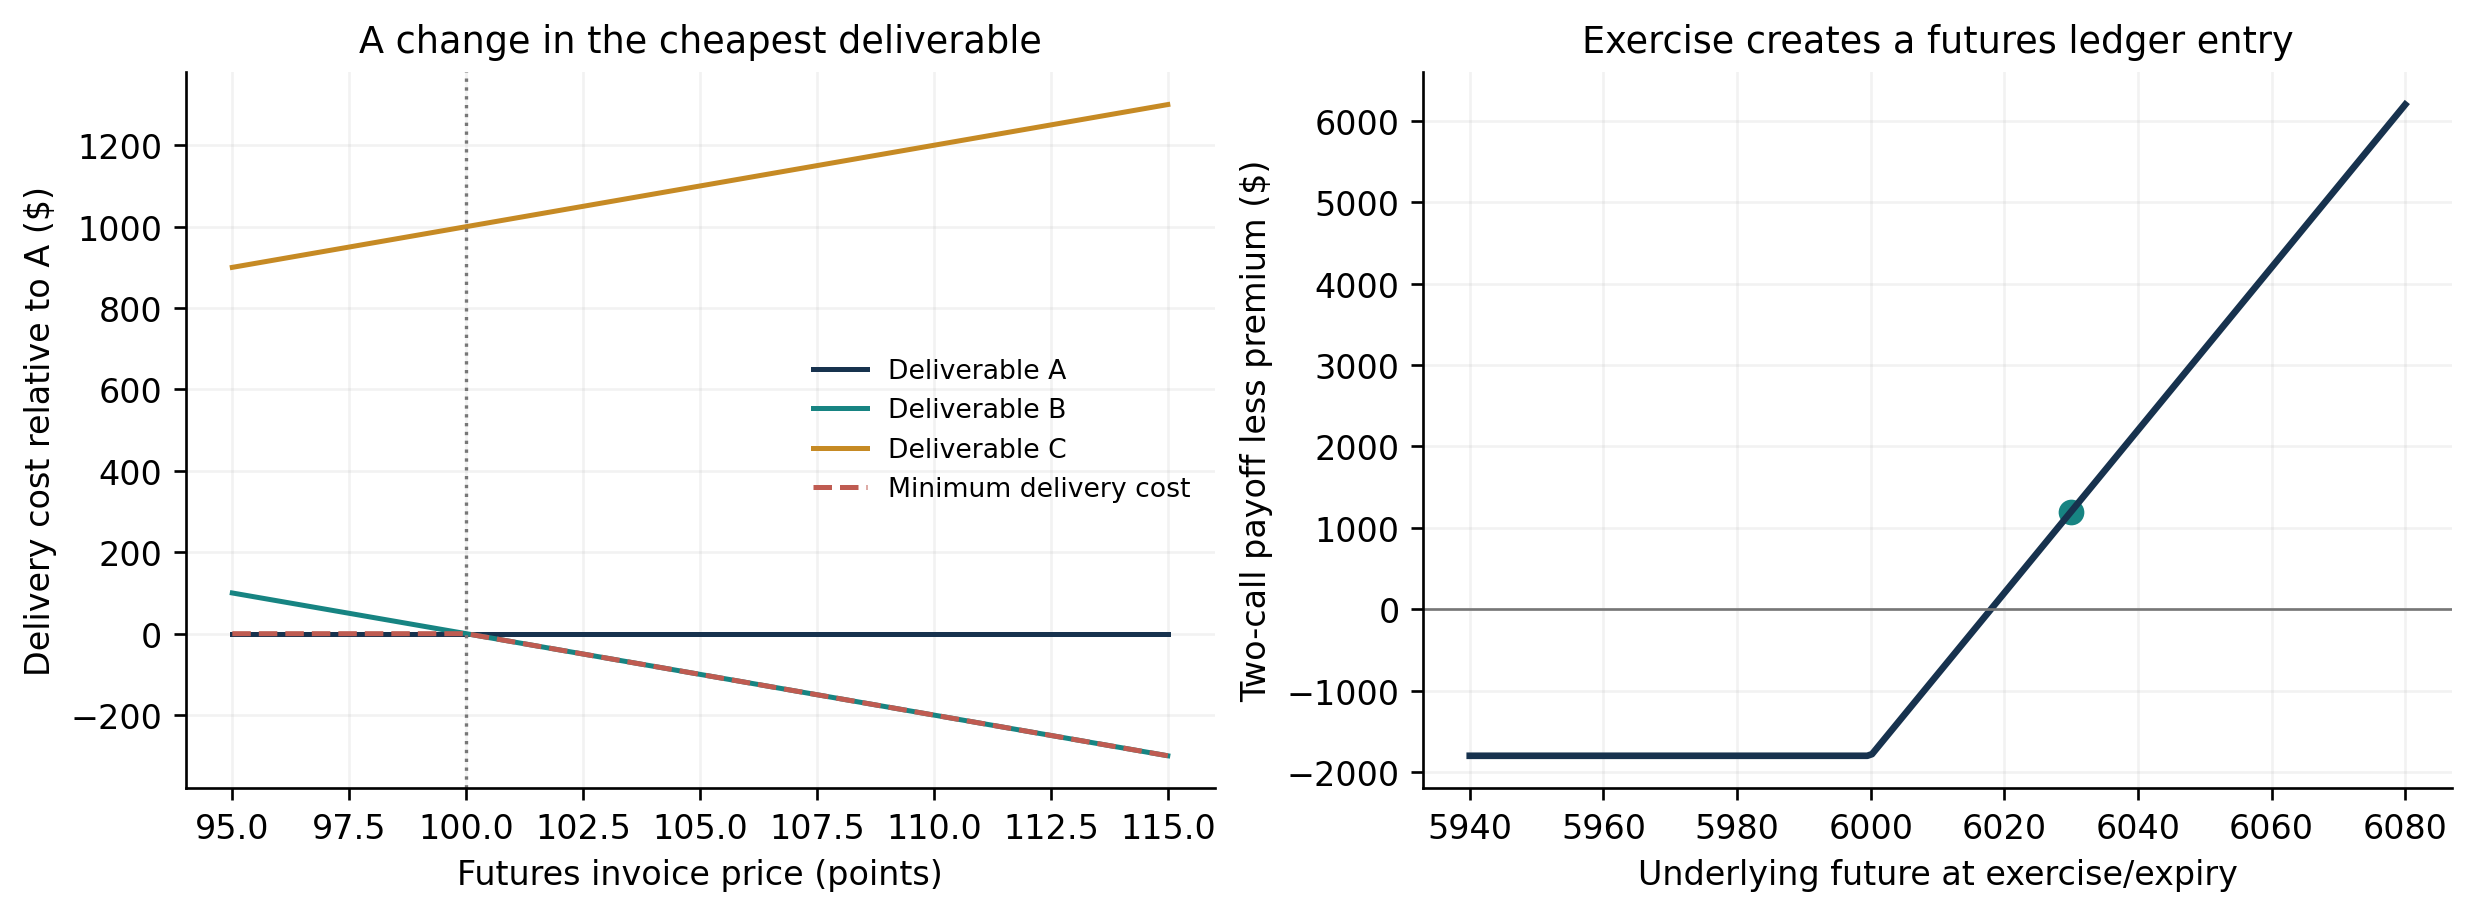
\includegraphics[width=\textwidth]{figures/09_delivery_options.png}
\caption{Two terminal maps. Left: synthetic delivery costs relative to deliverable A, preserving the identity of the cheapest security. Right: the intrinsic payoff less premium for the two calls in Example~\ref{ex:option}, assuming exercise or expiration and liquidation of any resulting futures at the displayed underlying value. Operational exercise conventions are specified separately from this payoff graph.}
\label{fig:delivery}
\end{figure}

\section{An integrated ledger and a default loss map}
\label{sec:ledger}

\subsection{From the depth walk to final cash}

We now connect the ten-contract ES depth walk to positions, variation, and collateral. Begin with \$12,000 cash and no positions. On day 1, execute the buy in Example~\ref{ex:depth}. On day 2, sell four contracts at 6,002. On day 3, sell the remaining six at 6,003. Daily settlements are respectively 6,001, 5,998, and 6,002. All numbers are synthetic.

For this ledger alone, assume a fixed requirement of \$1,000 posted cash per open contract, so the rule is $P_t=1000|z_t|$. This deliberately simple collateral rule is separate from the scenario-margin example. Assume the initial ten-contract margin can be posted from the starting cash before the first variation receipt, and later releases are available at the stated cycle. A different transfer schedule would change intracycle funding needs.

\begin{table}[htbp]
\centering\small
\begin{tabular}{@{}lrrrrrr@{}}
\toprule
Day & Settlement & Position & Variation & Margin change & Posted & Free cash\\
\midrule
0 & --- & 0 & --- & --- & 0 & 12,000.00\\
1 & 6,001 & 10 & 387.50 & 10,000 & 10,000 & 2,387.50\\
2 & 5,998 & 6 & $-700.00$ & $-4,000$ & 6,000 & 5,687.50\\
3 & 6,002 & 0 & 1,500.00 & $-6,000$ & 0 & 13,187.50\\
\bottomrule
\end{tabular}
\caption{A complete single-currency ledger. Monetary columns are dollars. Positive margin change is a transfer out of free cash into posted collateral. The margin rate is illustrative and is not an exchange quote.}
\label{tab:ledger}
\end{table}

The second-day variation is not $6\cdot50(5998-6001)$. Equation~\eqref{eq:vm} gives
\begin{equation}
 \mathrm{VM}_2=10\cdot50(5998-6001)
                   -4\cdot50(5998-6002)
              =-1500+800=-\$700.
\end{equation}
Similarly,
\begin{equation}
 \mathrm{VM}_3=6\cdot50(6002-5998)
                   -6\cdot50(6002-6003)
              =1200+300=\$1500.
\end{equation}
The position ends at zero, so Theorem~\ref{thm:telescoping} gives
\begin{align}
 \sum_t\mathrm{VM}_t
 &=50[4(6002)+6(6003)\notag\\
 &\hspace{20mm}-3(6000)-5(6000.25)-2(6000.50)]\notag\\
 &=\$1{,}187.50.
\end{align}
This agrees with $387.50-700+1500$ and with final cash minus initial cash. The \$10,000 initial margin is eventually released; it was never a \$10,000 trading loss.

\begin{figure}[htbp]
\centering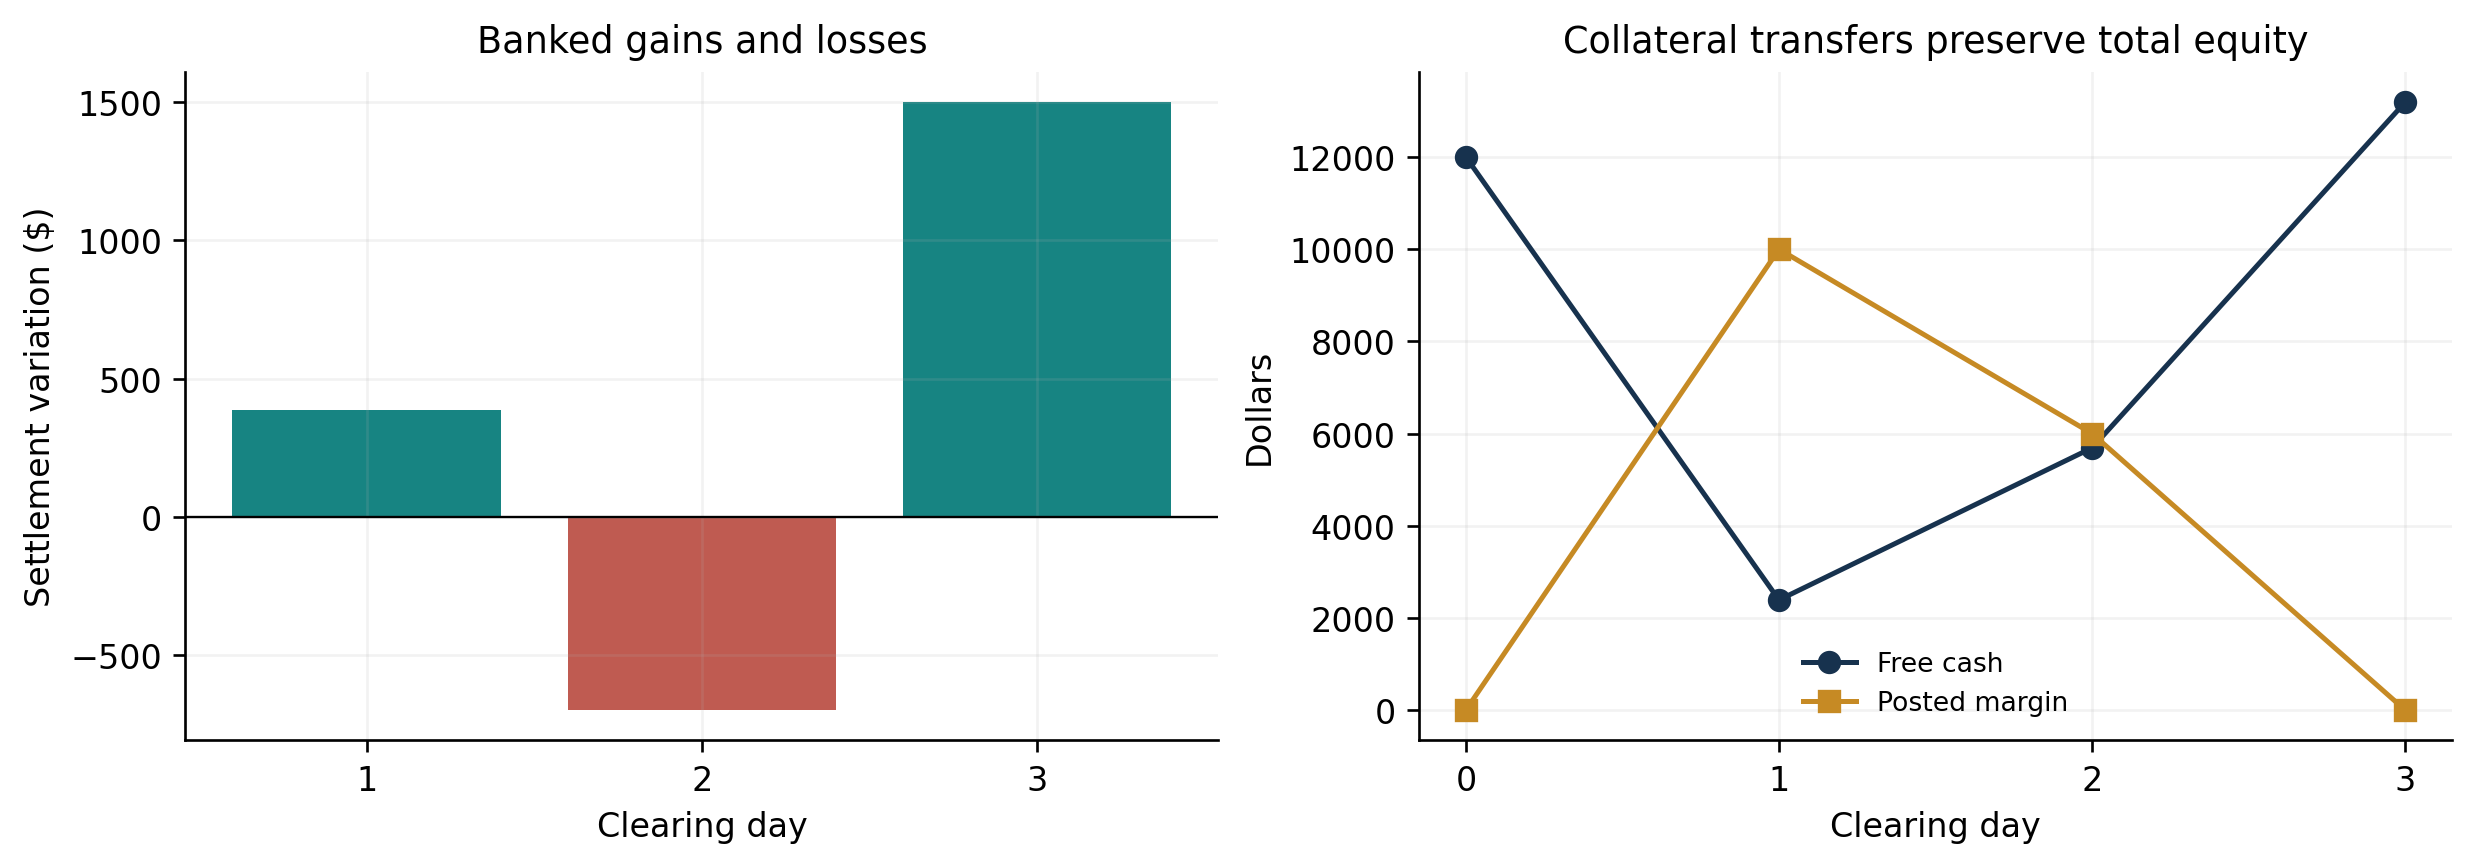
\includegraphics[width=\textwidth]{figures/06_settlement.png}
\caption{Cash flows and collateral in Table~\ref{tab:ledger}. Day 2 has negative variation but an increase in free cash because \$4,000 of posted margin is released. This is why a cash balance alone is not a P\&L series.}
\label{fig:ledger}
\end{figure}

The reconciliation uses the actual fills at their individual prices. Rounding the average fill to the nearest outright tick before calculating variation would alter the ledger. An average is a reporting summary; the trade records remain the accounting inputs.

\subsection{A default waterfall is another ordered allocation}

CME's public safeguards architecture places defaulter resources before the clearinghouse contribution, mutualized guaranty resources, and assessment powers \citep{CMESafeguards}. Account segregation and the applicable clearing service determine which resources are available. The following is an abstract loss-allocation model of that ordered structure, with no production dollar amounts or legal recovery rules inferred.

Let $L\ge0$ be a loss to absorb and $r_1,\ldots,r_k\ge0$ the resources available in the applicable order. Define
\begin{equation}
 d_i(L)=\min\left\{r_i,\left(L-\sum_{j<i}r_j\right)_+\right\},
 \qquad U(L)=\left(L-\sum_{i=1}^kr_i\right)_+.
\label{eq:waterfall}
\end{equation}

\begin{proposition}[Ordered loss conservation]
The draws in \eqref{eq:waterfall} satisfy $0\le d_i\le r_i$ and
\begin{equation}
 \sum_id_i(L)+U(L)=L.
\end{equation}
Each draw is continuous, nondecreasing, and piecewise linear in $L$. The first positive draw from layer $i$ occurs only after earlier resources are exhausted.
\end{proposition}
\begin{proof}
Represent each resource layer by a consecutive interval of length $r_i$. Its draw is the intersection length with $(0,L]$, exactly as in the FIFO prefix proof. The intersections partition the absorbed loss, and the portion beyond all intervals is $U(L)$.
\end{proof}

In synthetic millions of dollars, resources $(8,2,5,4)$ and loss 17 produce draws $(8,2,5,2)$ with no residual. The same arithmetic as FIFO appears because both allocate an amount through an ordered list of capacities. The economic interpretations differ: one allocates contracts to resting orders, the other losses to legally available resources.

Nominal capacity does not establish time availability. A future assessment may absorb an ultimate loss while failing to provide cash for an earlier settlement deadline. The funding theorem and the waterfall model therefore answer different questions: when cash is available, and whose resources absorb the loss.

\subsection{Reproducibility and the scope of verification}

The source project includes \texttt{reproduce.py} and nine PNG figures. Numerical outputs and runtime versions are recorded in \texttt{results.json} and \texttt{environment.json}. The script verifies 63 numerical result groups, including exact allocation vectors, the shared-capacity bound, opening cases, rounded values, the complete cash ledger, the margin counterexample, funding prefixes, option cash, delivery invoices, and waterfall draws. It also checks allocation conservation and discrepancy over 84 declared quantity, demand, and threshold combinations.

Fractions are used for proportional entitlements and price arithmetic; decimal arithmetic implements monetary rounding. A continuous linear program verifies the implied-resource upper bound, which is also certified analytically by Proposition~\ref{prop:dual}. All figures use deterministic synthetic inputs. There is no statistical fitting or Monte Carlo error.

These checks validate the published examples and modeled invariants. They do not certify product conformance, a live feed decoder, a production margin model, or a trading strategy. The source register identifies the operational documents and the part of each used in the manuscript.
\FloatBarrier

\section{Conclusion}

The mathematics of a listed derivatives market is organized by the objects its rules transform. An allocation map consumes resting quantity and assigns fills. A leg map converts strategy trades into signed positions. A resource matrix prevents double use of orders supporting implied opportunities. An observation map determines which aspects of those mechanisms are visible. Opening and settlement rules select prices for different purposes. A monetary-value map translates positions and trades into exact variation. Margin and collateral maps determine whether the resulting positions can be maintained. Exercise and delivery create or discharge additional obligations.

Several conclusions follow from keeping those maps separate. Integer pro-rata allocation need not compose across events. Implied quantities need not add. An MBO sequence need not imply FIFO execution. A futures quote-value integral is not an upfront purchase payment. Terminal profit does not determine peak funding. Convex portfolio risk can rise when one hedge leg is removed. Enough aggregate collateral value does not guarantee enough settlement cash. A final futures mark and a physical invoice are different ledger entries.

The framework's mathematical building blocks are deliberately transparent. Prefix geometry establishes FIFO and waterfall conservation. Convexity describes depth costs and the declared scenario-risk model. Linear constraints and dual certificates expose shared-resource bottlenecks. Telescoping identifies exact settlement totals; prefix maxima identify their funding requirements. None of these tools removes the need to specify the contract, market phase, account, and operative rule branch.

Further work can add empirical event intensities, full product configurations, calibrated option repricing, a complete implied-recipe priority engine, and time-dependent collateral transformation. Such extensions should preserve the distinctions and reconciliations established here. A more realistic model is useful only if its additional detail enters the correct part of the lifecycle.

\FloatBarrier
\clearpage
\begingroup\small
\bibliographystyle{plainnat}
\bibliography{references}
\endgroup
\appendix
\clearpage
\section{Implementation boundaries and numerical reference}

\subsection{What is exact in the supplied implementation}

The FIFO routine consumes an ordered list. The proportional routine calculates rational entitlements, applies an integer minimum, and allocates residual demand FIFO. Both operate on the ordinary-order state declared in Section~\ref{sec:allocation}. They do not infer TOP status, LMM entitlements, hidden replenishment, or a product's configured sequence. The opening routine covers the five tabulated tie cases and the unique-volume case; no production fallback is supplied for remaining exact ties.

The normal money-value map uses decimal half-away-from-zero rounding at one-contract value level. No special notional rounding, inverse currency conversion, option futures-style premium, or daily-value adjustment is applied. The numerical examples explicitly choose instruments and conventions for which the shown arithmetic is consistent with the declared map.

The margin routine uses exactly the six vectors and three additions in Section~\ref{sec:margin}. The plotting grid is continuous, while the example positions are integer contracts. The collateral example uses one legal account, fractional bond-value allocation, a synthetic haircut, and a cash-only current variation obligation. Extending it across accounts or currencies requires additional constraints.

\begin{table}[htbp]
\centering\small
\begin{tabularx}{\textwidth}{@{}lX@{}}
\toprule
Quantity & Reproduction target\\
\midrule
37-lot allocation & FIFO $(12,25,0)$; PR/FIFO $(5,10,22)$\\
4-lot fragmentation & One event $(2,0,2)$; two 2-lot events $(2,2,0)$\\
ES depth walk & Average 6000.225; shortfall \$112.50\\
Shared implication & Individually $5+6$; jointly at most 8\\
Completion indices & FIFO $(1,2,3)$; PR/FIFO $(3,3,3)$\\
Opening price & 102, with 10 matched contracts\\
VWAP perturbation & 6000.25 to $6000.423076\ldots$; rounded mark 6000.50\\
Three-day variation & \$387.50, $-\$700.00$, \$1,500.00\\
Total cash gain & \$1,187.50; final cash \$13,187.50\\
Illustrative margin & \$11,200 at $(5,-5)$; \$12,800 at $(5,-3)$\\
Peak funding & \$10,000 versus zero; \$15,000 with margin shock\\
Collateral bottleneck & \$23,000 credited value; only \$5,000 current cash\\
Option example & $-\$1,800$ premium; \$3,000 variation; \$1,200 net\\
Delivery comparison & Net costs \$0, $-\$200$, \$1,200; B cheapest at 110\\
Waterfall & Loss 17; draws $(8,2,5,2)$ in synthetic millions\\
\bottomrule
\end{tabularx}
\caption{Principal numerical checkpoints. Each belongs to its stated model; the margin and collateral examples are separate from the fixed-rate integrated ledger.}
\end{table}

\subsection{Source dating and reproducible compilation}

The manuscript date and consultation date are September 11, 2026 (UTC). A 2026 bibliography year for a continuously maintained operational page records the consulted snapshot; it does not imply original publication in that year. The money-calculation specification retains its stated 2015 document year. Source URLs, titles, and consultation notes are supplied in the bibliography and in \texttt{source\_register.md}.

Compile \texttt{The\_Mathematics\_of\_CME.tex} with pdfLaTeX in Overleaf. Included figures require no Python or shell escape. To regenerate them and the numerical ledger, run \texttt{reproduce.py}. The source archive includes a SHA256 manifest.
\FloatBarrier

\end{document}
